\chapter{Prezentarea aplicației}

OfOps este o aplicație WEB concepută pentru simplificarea procesului de rezervare a diferitelor resurse dintr-un mediu de lucru. Indiferent dacă aveți nevoie să vă asigurați un loc de parcare, să rezervați un birou pentru o anumită perioadă de timp sau o sală de ședință, OfOps vine în ajutorul tău!

\section{Flow-ul aplicației}

Navigarea pe OfOps urmează următorul curs:

\begin{figure}[!htb]
    \centering
    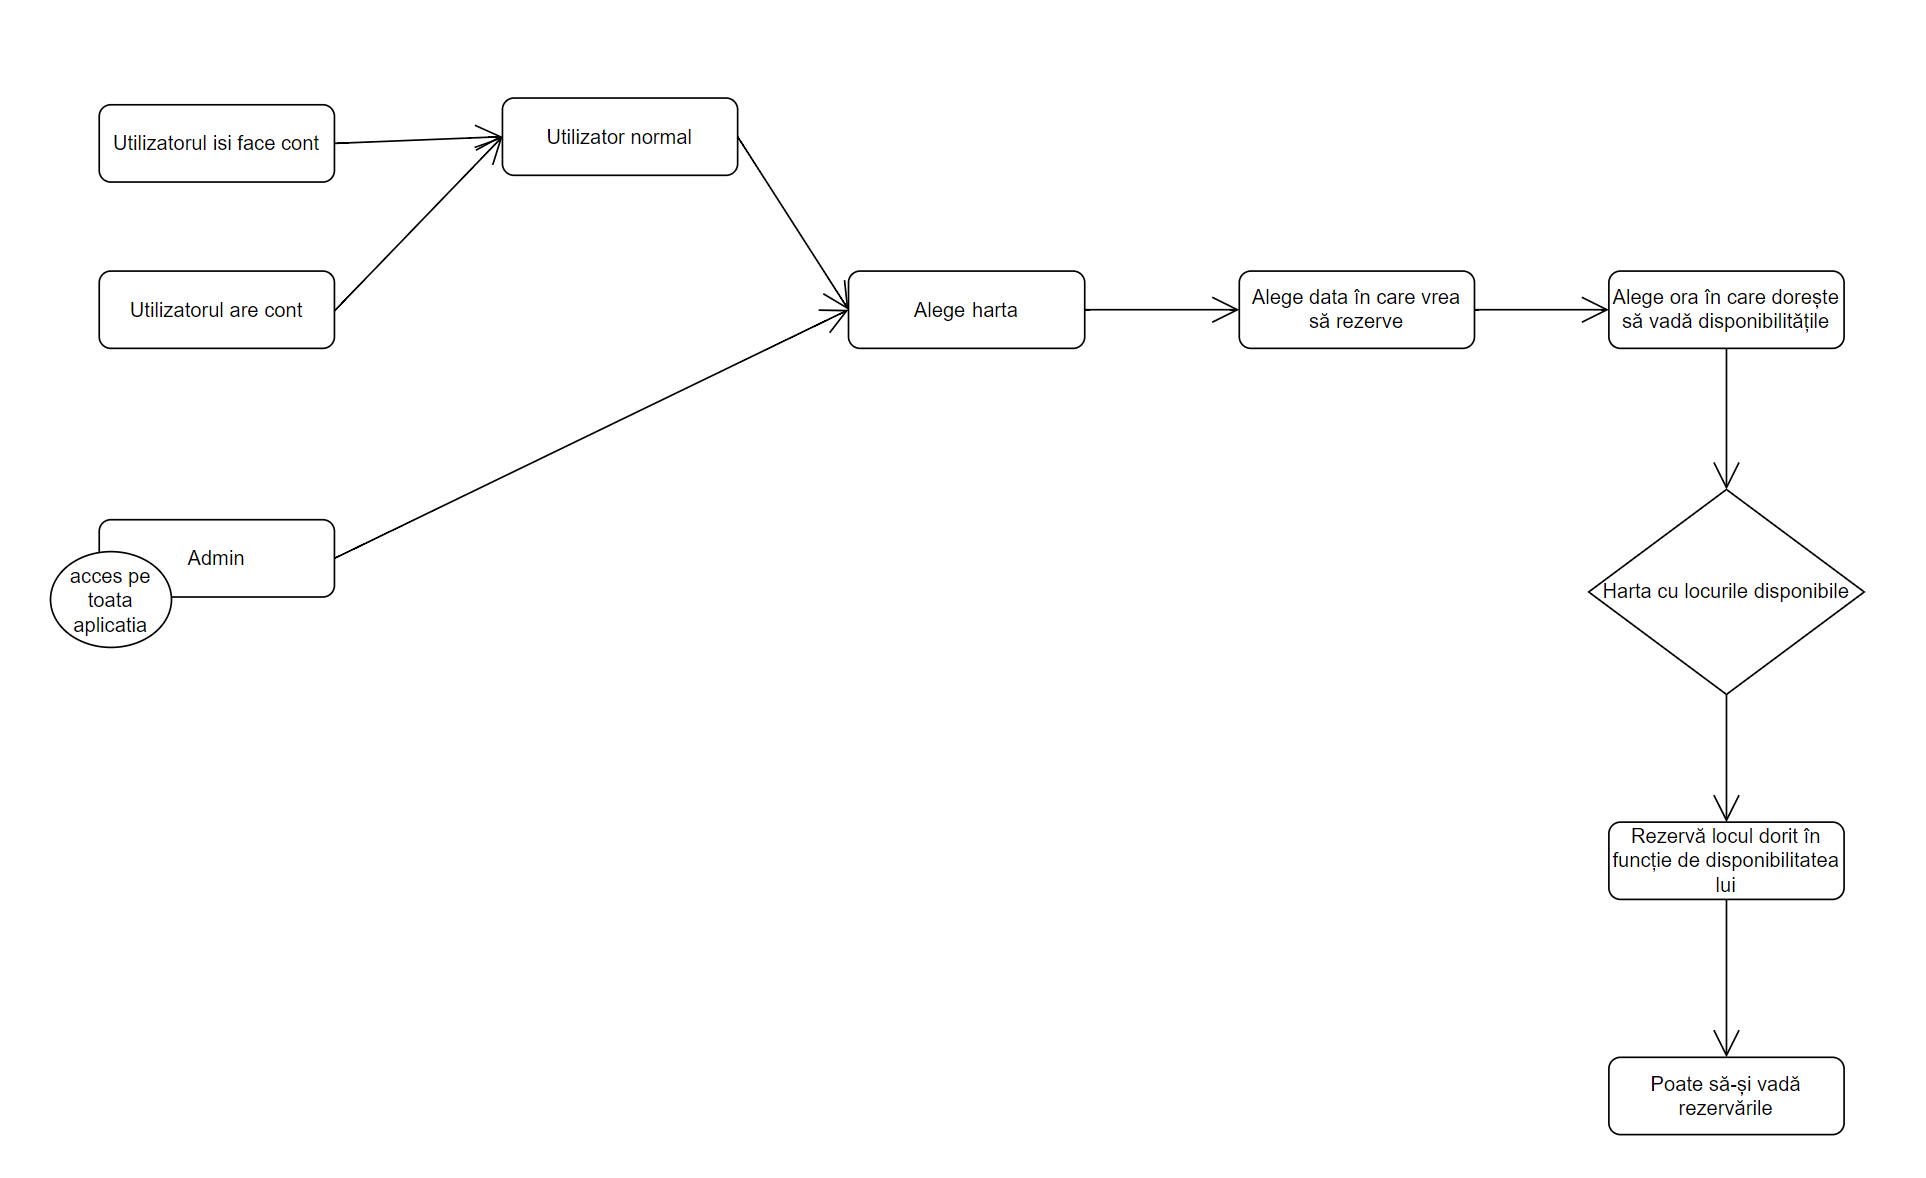
\includegraphics[width=0.9\linewidth]{images/flow.png}
    \caption{Flow OfOps}
    \label{fig:flow}
\end{figure}

\newpage

\section{Diagrama E/R}

\begin{figure}[!htb]
    \centering
    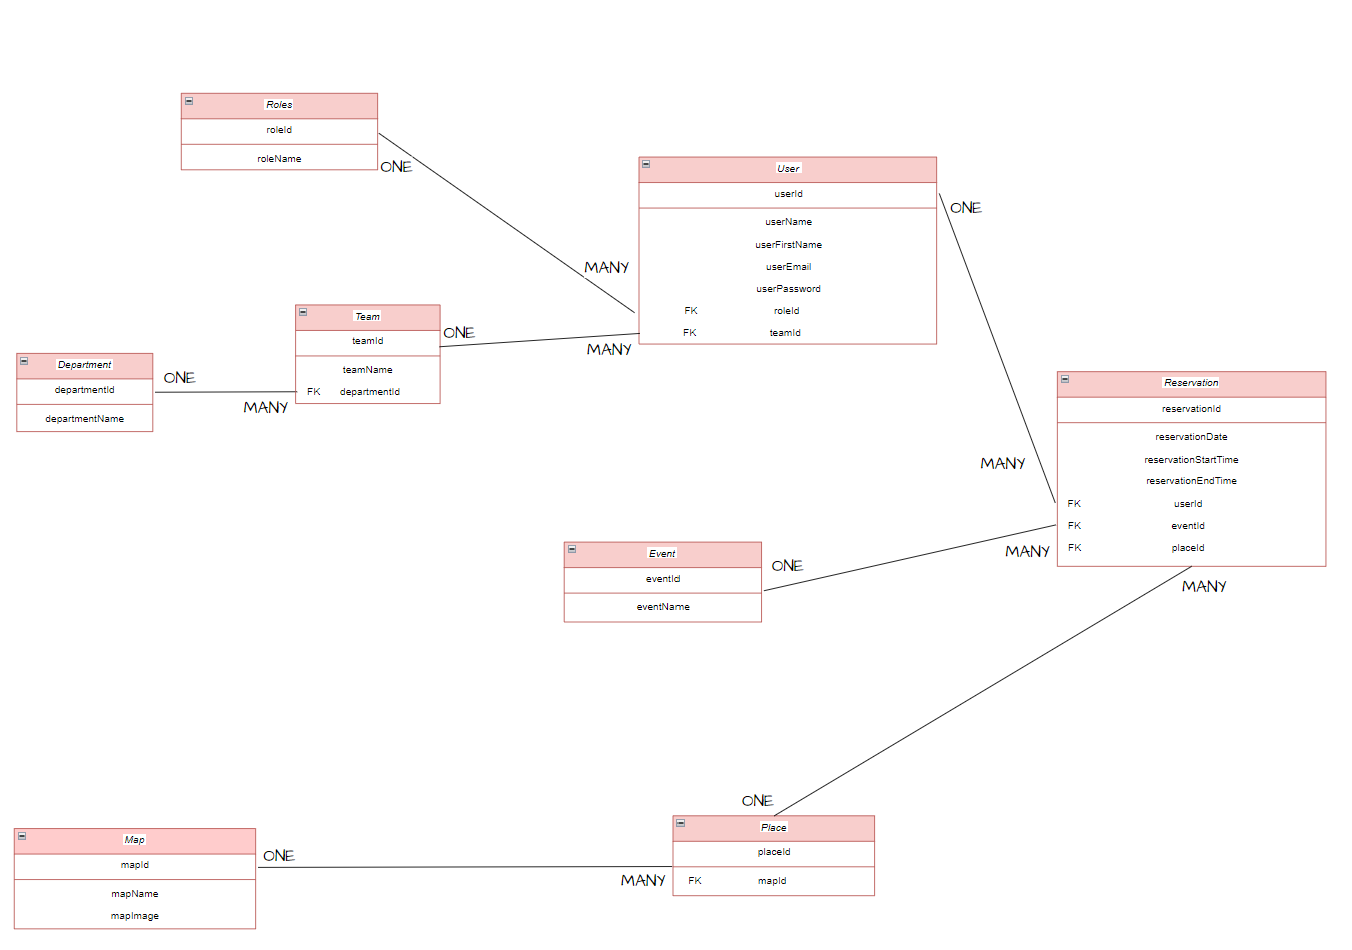
\includegraphics[width=0.9\linewidth]{images/diagrama.png}
    \caption{Diagrama E/R}
    \label{fig:diagrama}
\end{figure}

\section{Pagina principală și mențiuni generale}

Pagina principală este cea care întâmpină utilizatorul în momentul în care navighează pentru prima oară pe ea. Aceasta oferă opțiuni limitate utilizatorului și anume cele de \textbf{Login} și \textbf{Create an account}.

\begin{figure}[!htb]
    \centering
    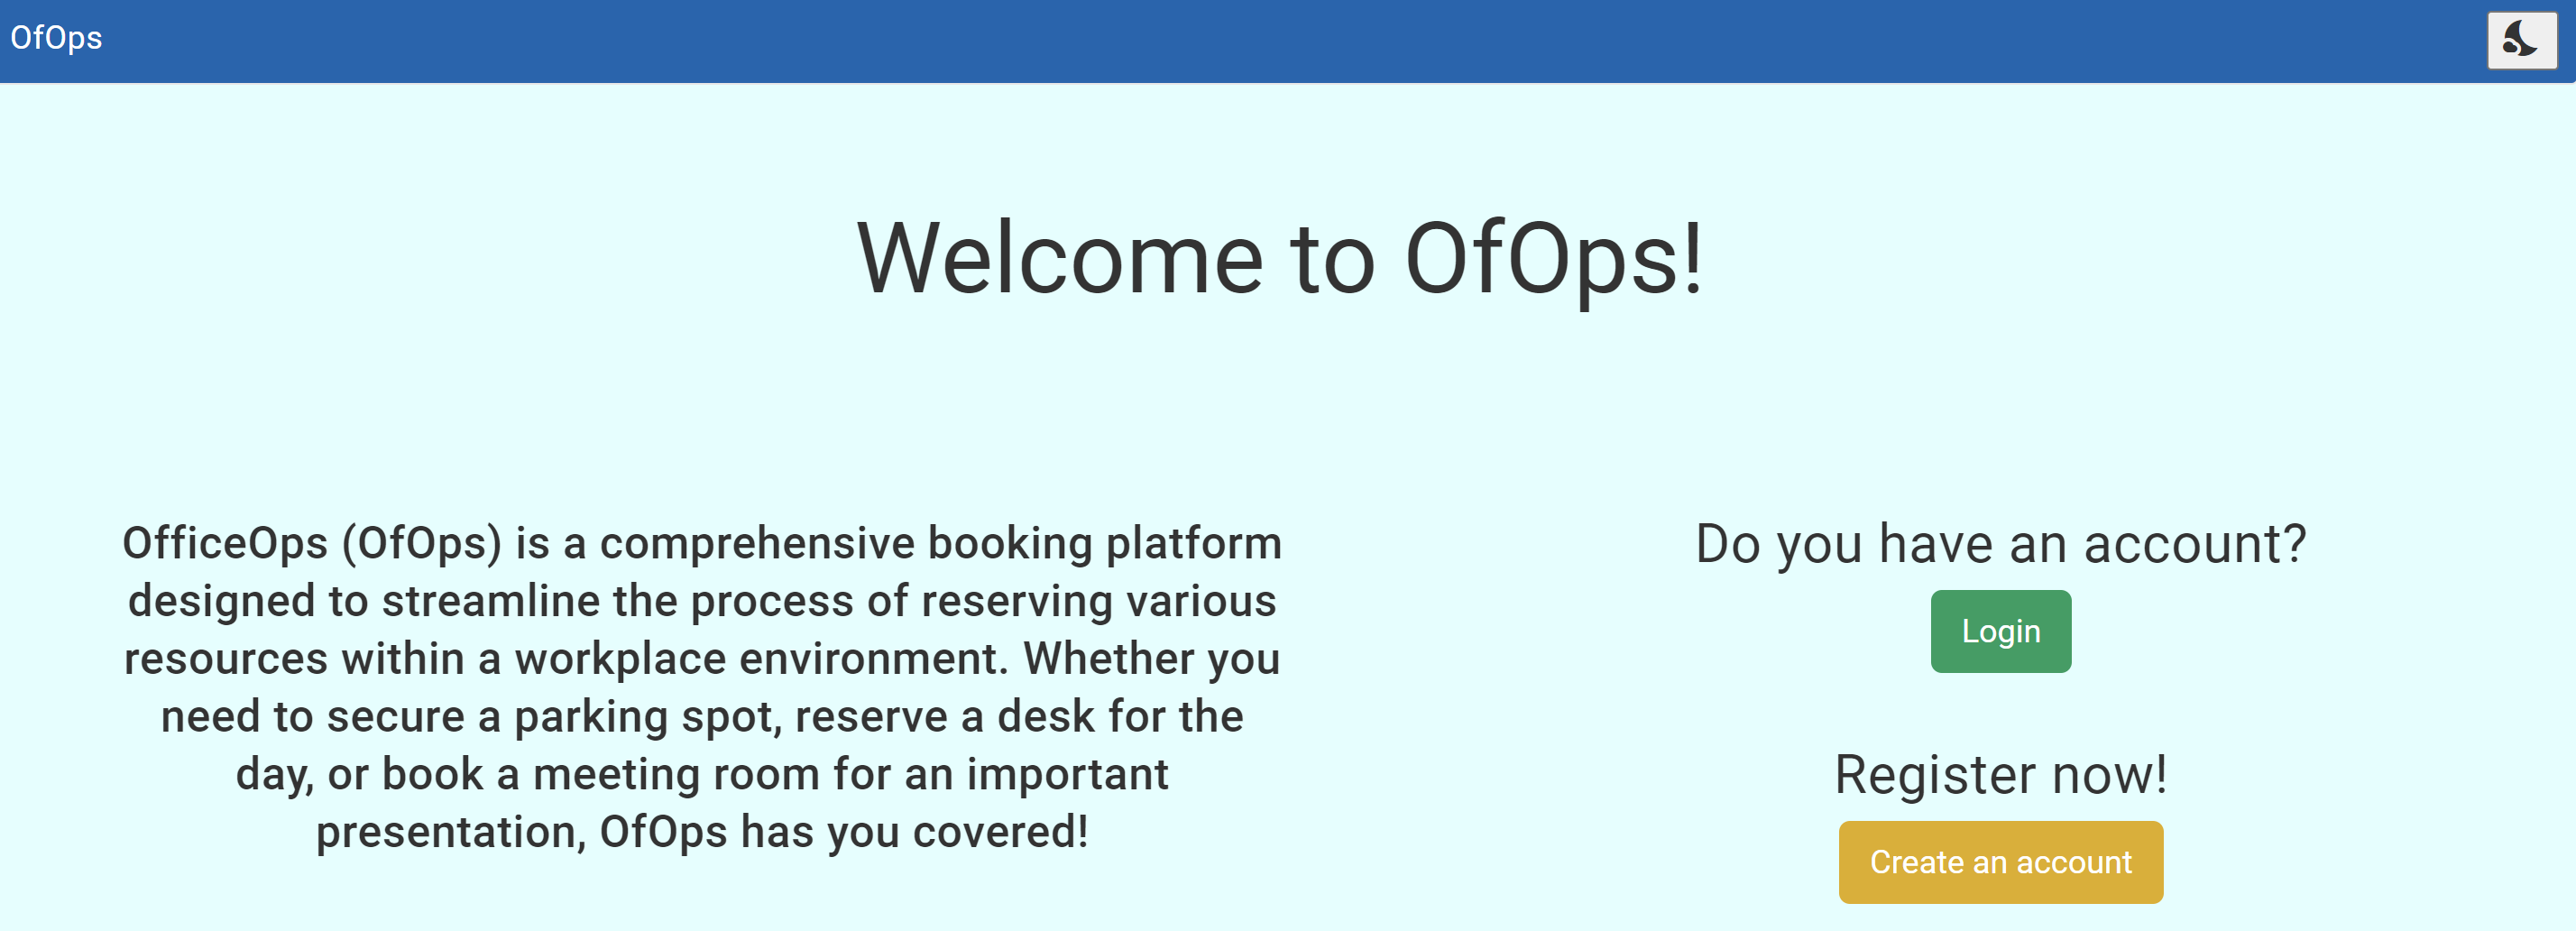
\includegraphics[width=0.9\linewidth]{images/pagina-nelogat.png}
    \caption{Pagina principală}
    \label{fig:principal}
\end{figure}

De asemenea, OfOps dispune și de varianta pentru dark mode. Această opțiune, cunoscută și sub denumirea de night mode, a devenit populară în ultimii ani, mai exact, din anul 2019 în care Google a introdus-o pe Android OS, fapt ce i-a făcut pe toți giganții din industria IT să-i urmeze modelul.\cite{citation9} Posibilitatea utilizatorului de alege modul de navigare pe aplicație denotă prioritizarea dorințelor acestuia, rezultâand, astfel, o experiență mult mai plăcută pentru el. Schimbarea la dark mode se realizează prin apăsarea butonului din dreapta sus a paginii.

\begin{figure}[!htb]
    \centering
    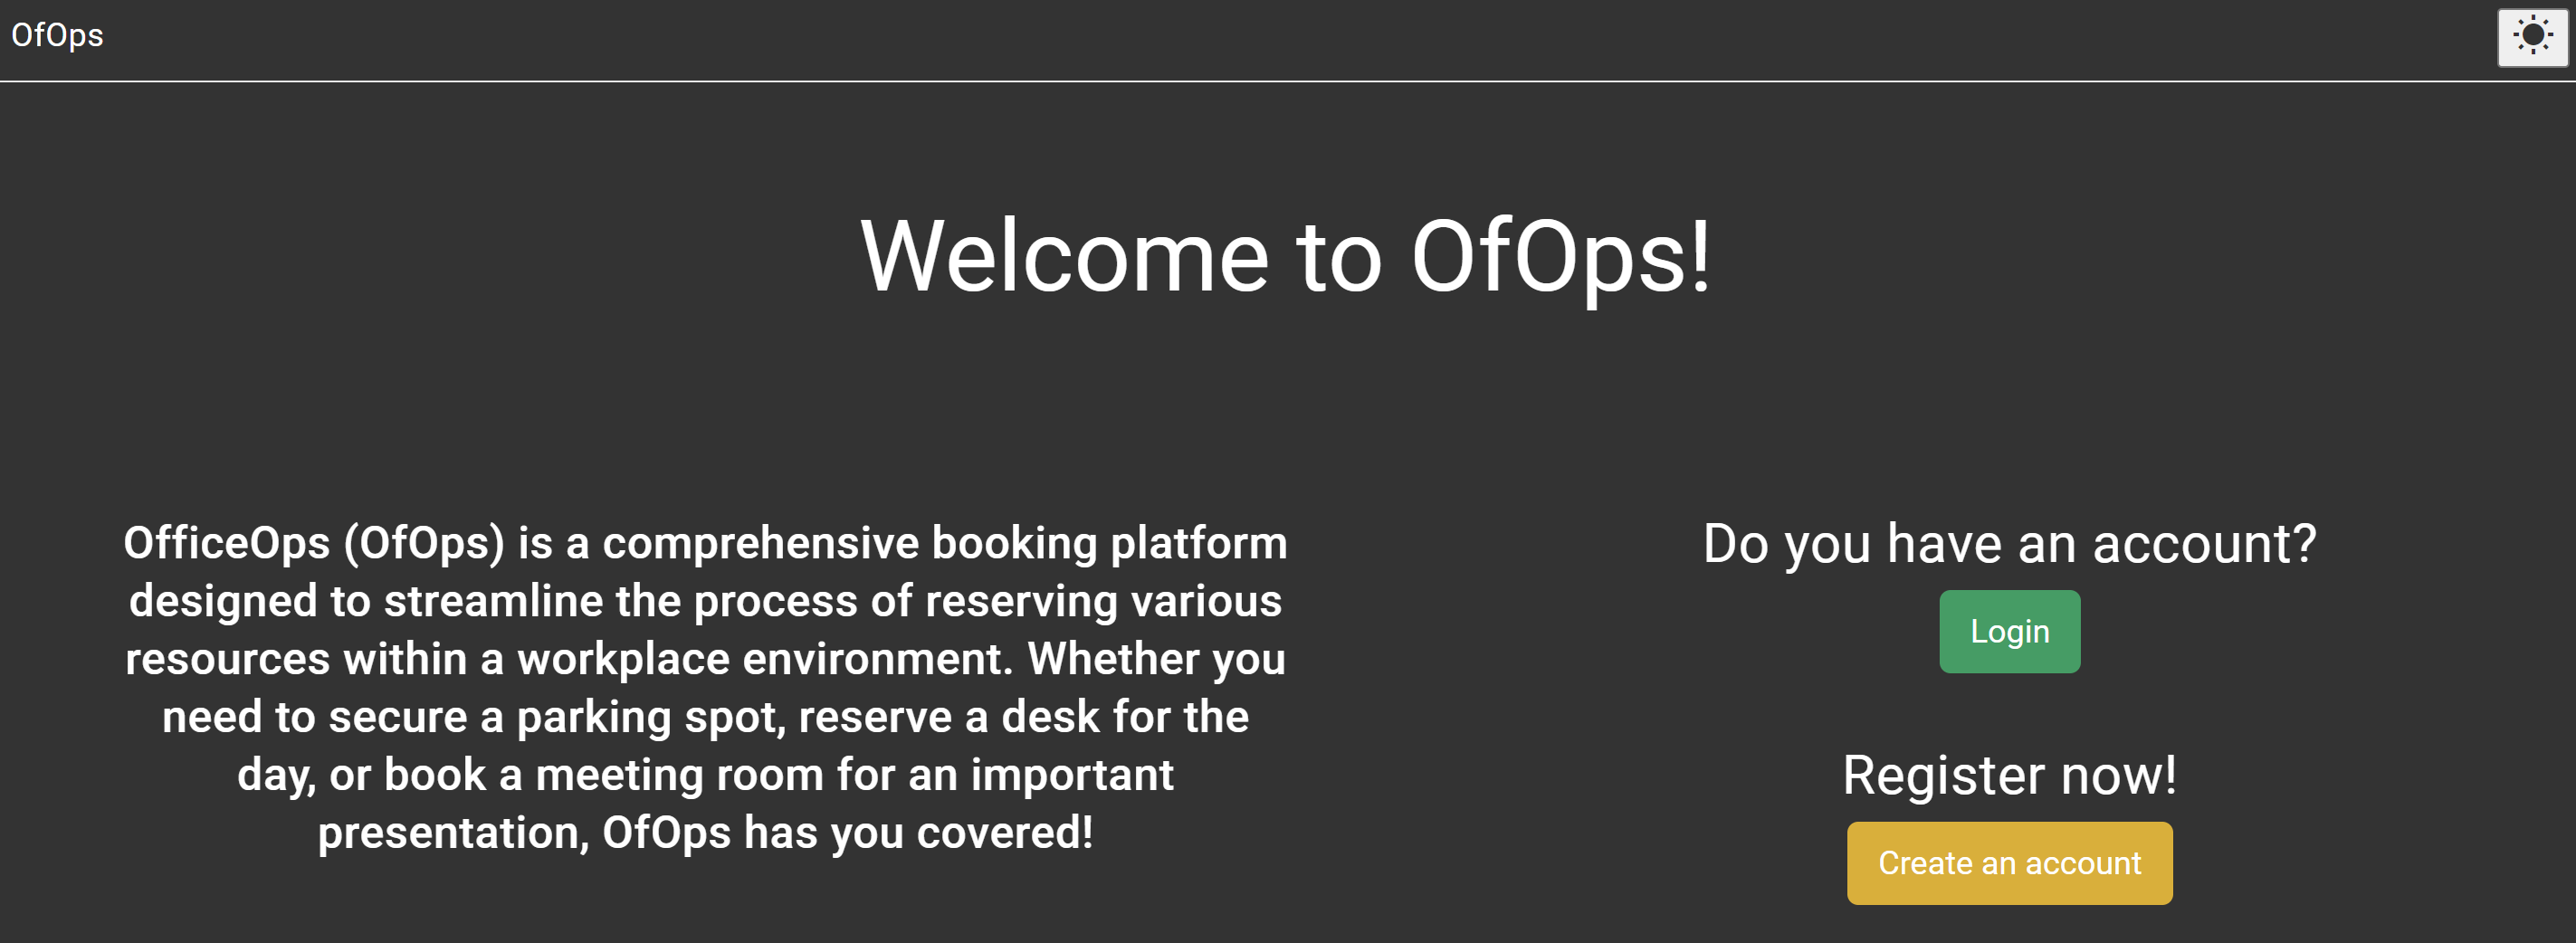
\includegraphics[width=0.9\linewidth]{images/dark.png}
    \caption{Dark mode}
    \label{fig:dark}
\end{figure}

\section{Pagina de înregistrare a unui utilizator}

Pagina de înregistrare a unui utilizator este disponibilă în momentul click-ului pe butonul \textbf{Create an account} din pagina principală. Utilizatorul este redirecționar către formularul de creare a unui cont.  

\begin{figure}[!htb]
    \centering
    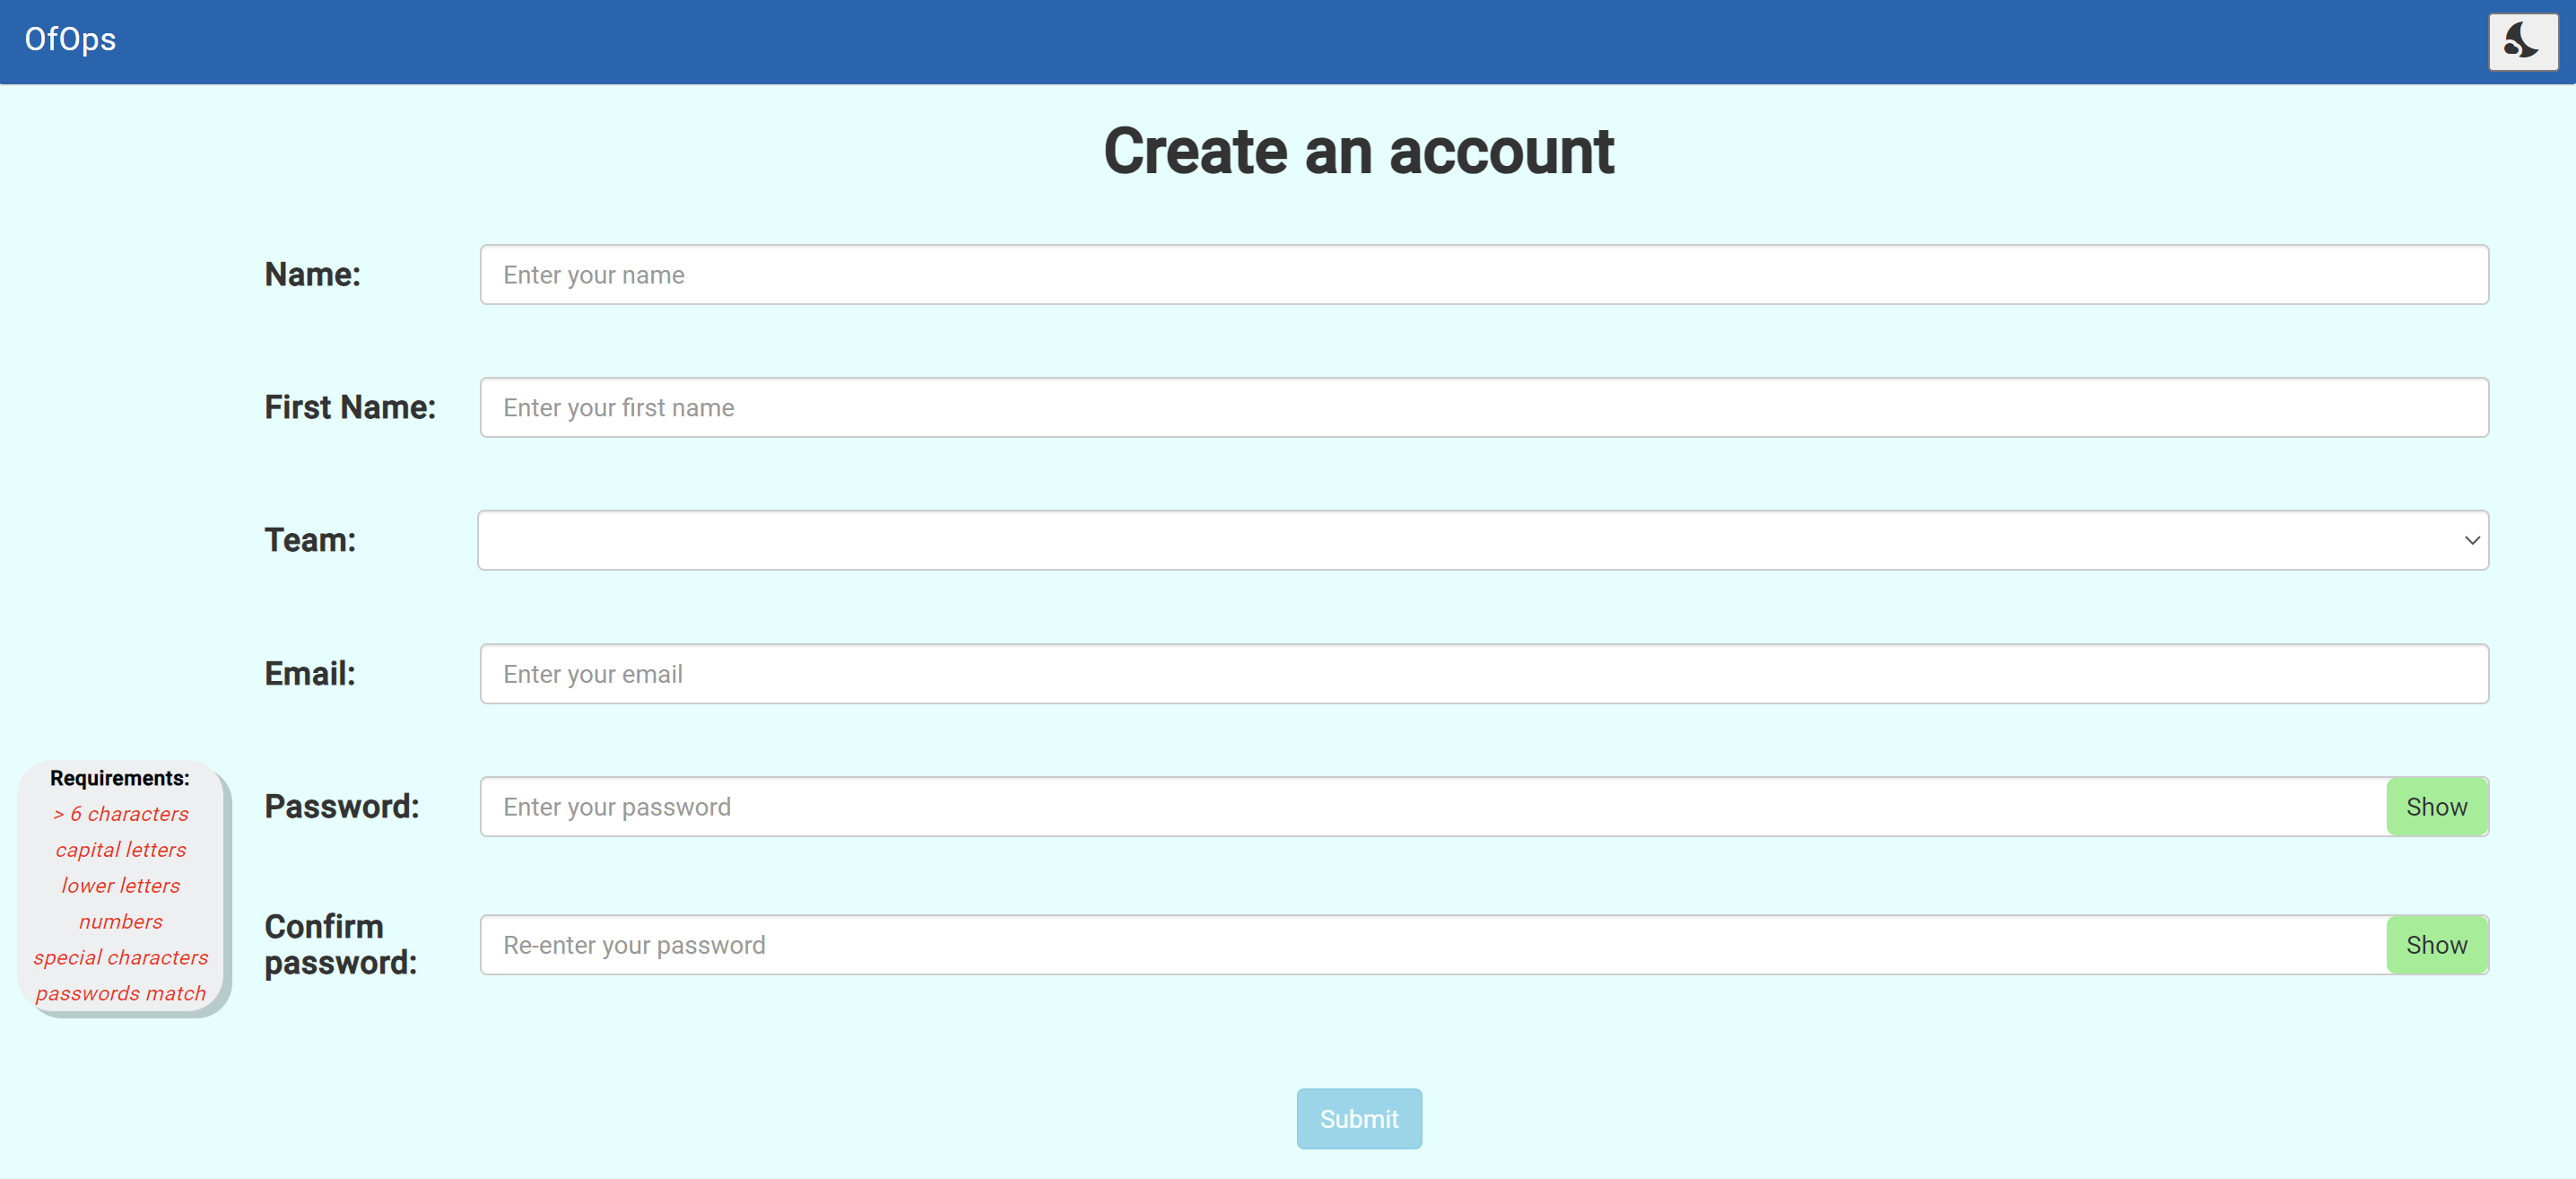
\includegraphics[width=0.9\linewidth]{images/inregistrare.png}
    \caption{Înregistrarea pe OfOps}
    \label{fig:inregistrare}
\end{figure}

Crearea unui cont se realizează pein completarea tuturor câmpurilor. Acestea au implementate validări pe care dacă user-ul nu le îndeplinește va duce la inactivarea butonului de submit. În caz contrar, butonul se va activa. De asemenea, există un set de reguli pentru parolă, astfel încât aceasta să fie cât mai greu de spart. Utlizitatorul are posibilitatea să își vadă parola în cazul în care nu se potrivește cu cea trecută la \textbf{Confirm password}.

\begin{figure}[!htb]
    \centering
    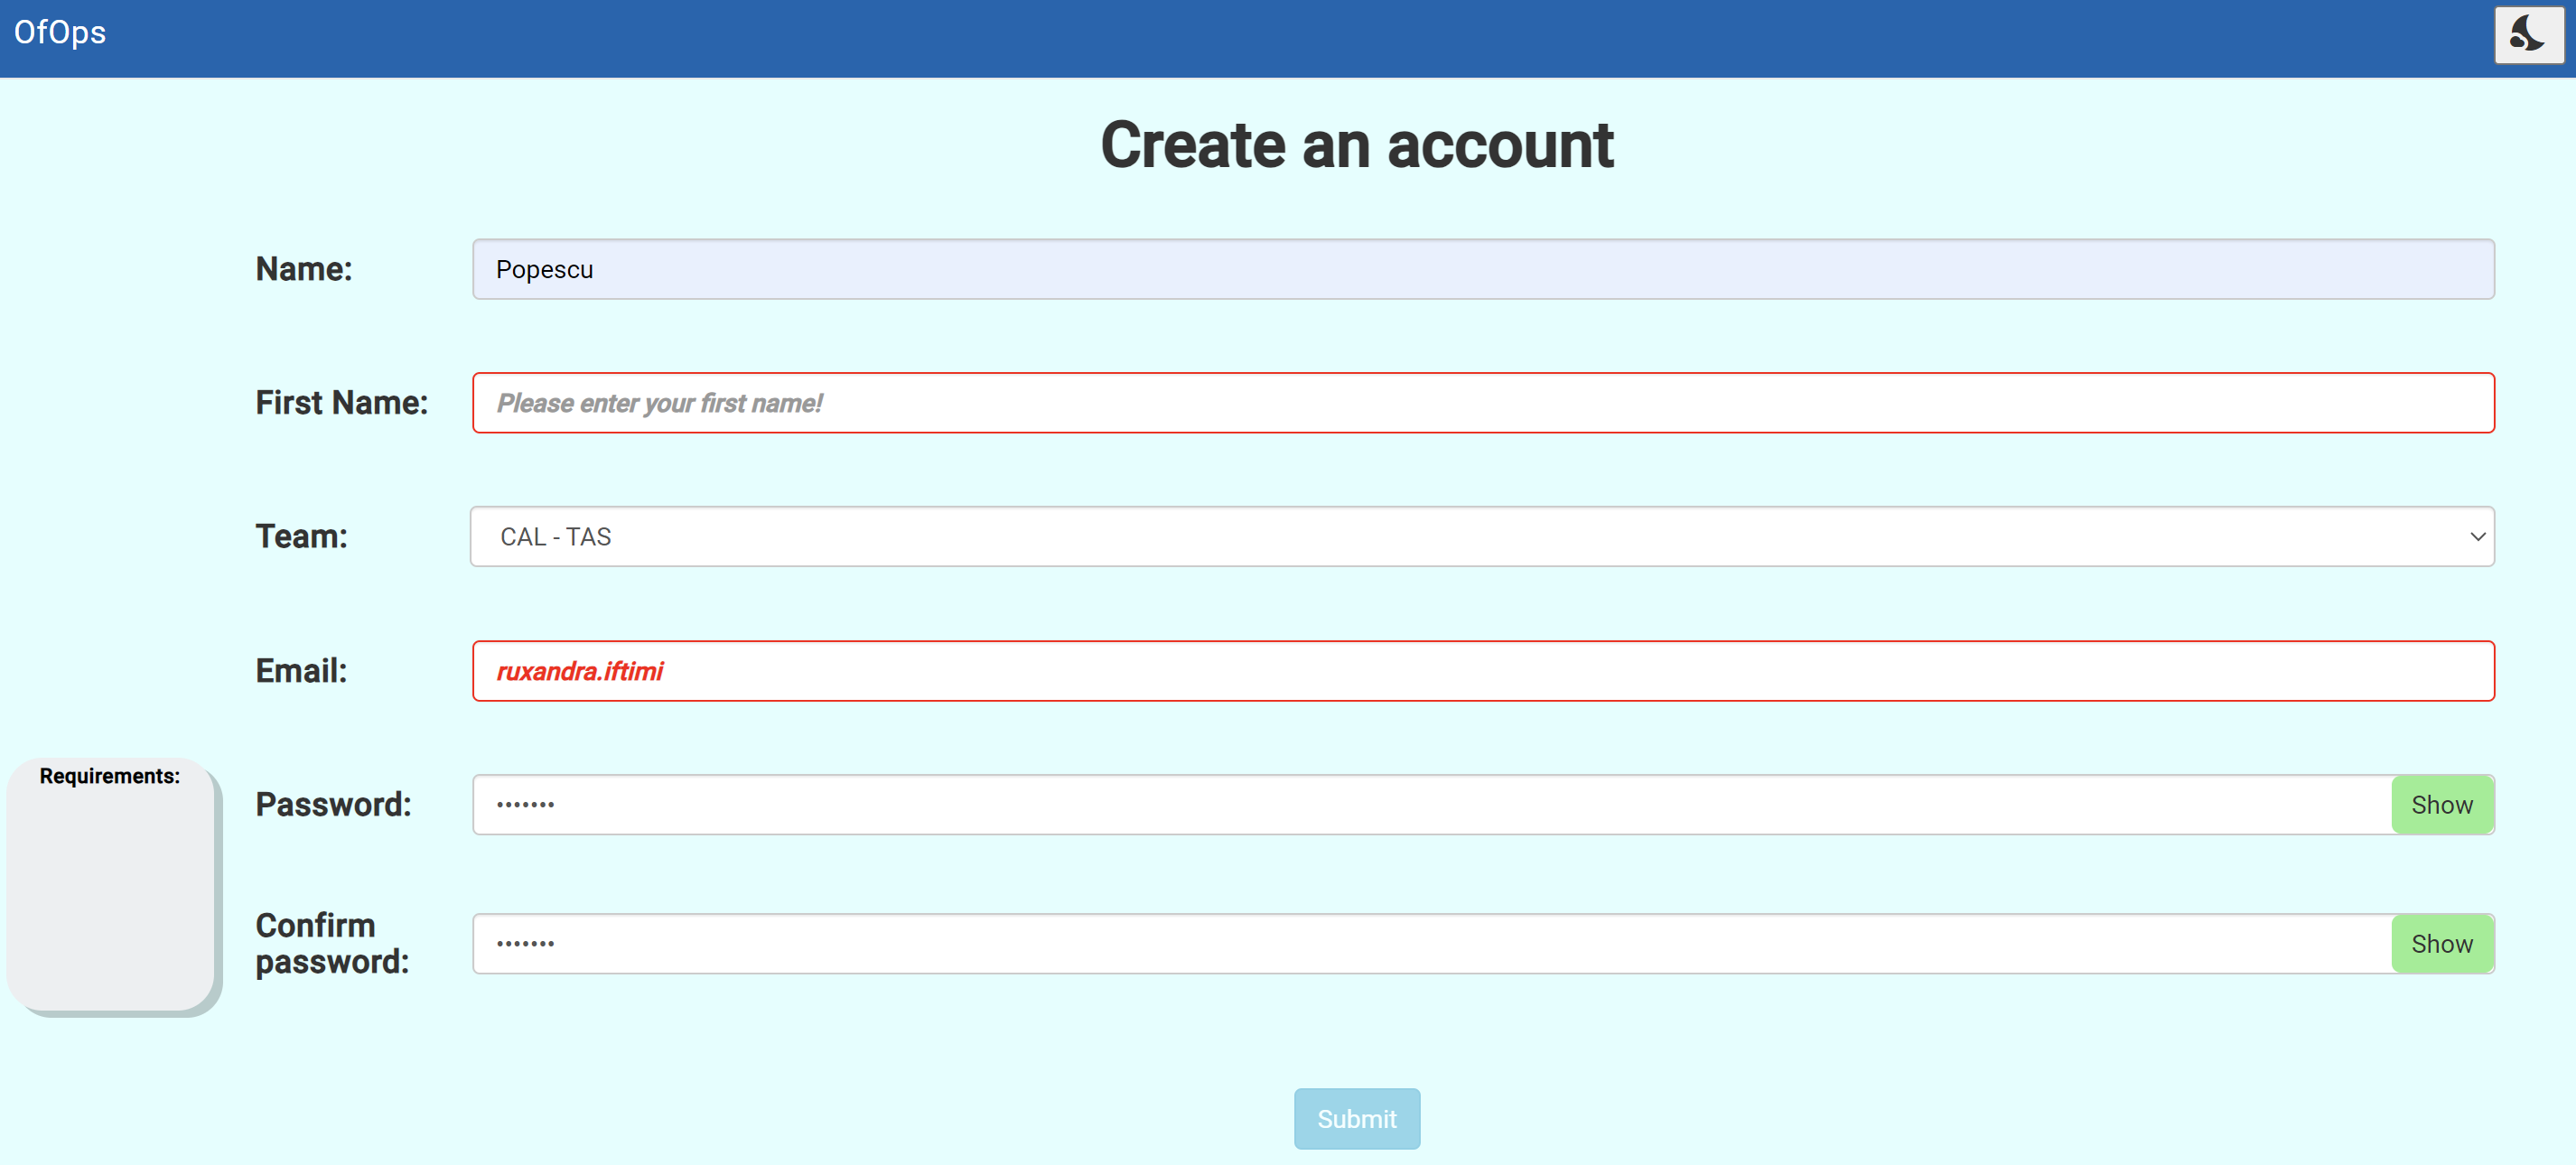
\includegraphics[width=0.9\linewidth]{images/greseli.png}
    \caption{Validările câmpurilor nu sunt respectate}
    \label{fig:greseli}
\end{figure}

La apăsarea butonului de \textbf{Submit}, user-ul va fi redirecționat către pagina de \textbf{Sign in}, primind un pop-up legat de viitoarea autentificare în aplicație.  

\begin{figure}[!htb]
    \centering
    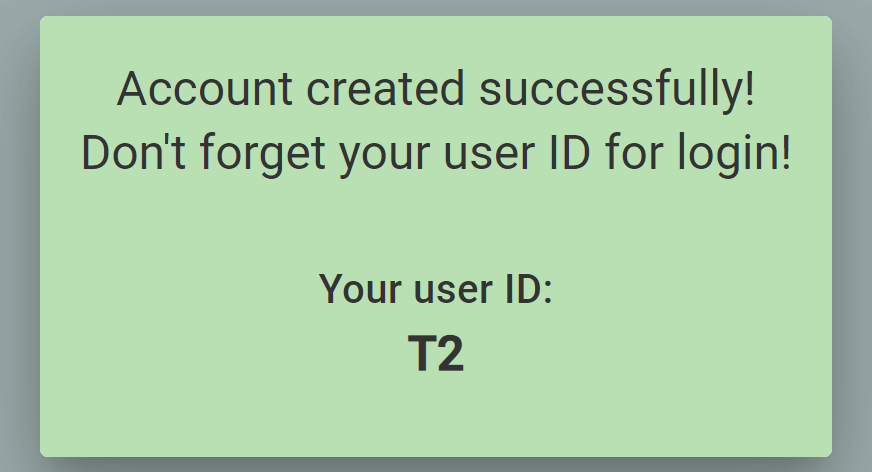
\includegraphics[width=0.9\linewidth]{images/autentf.png}
    \caption{Înregistrare reușită}
    \label{fig:autentf}
\end{figure}

\section{Pagina de sign in}
Pagina de \textbf{Sign in} este locul în care utilizatorul se loghează pe OfOps. 

\begin{figure}[!htb]
    \centering
    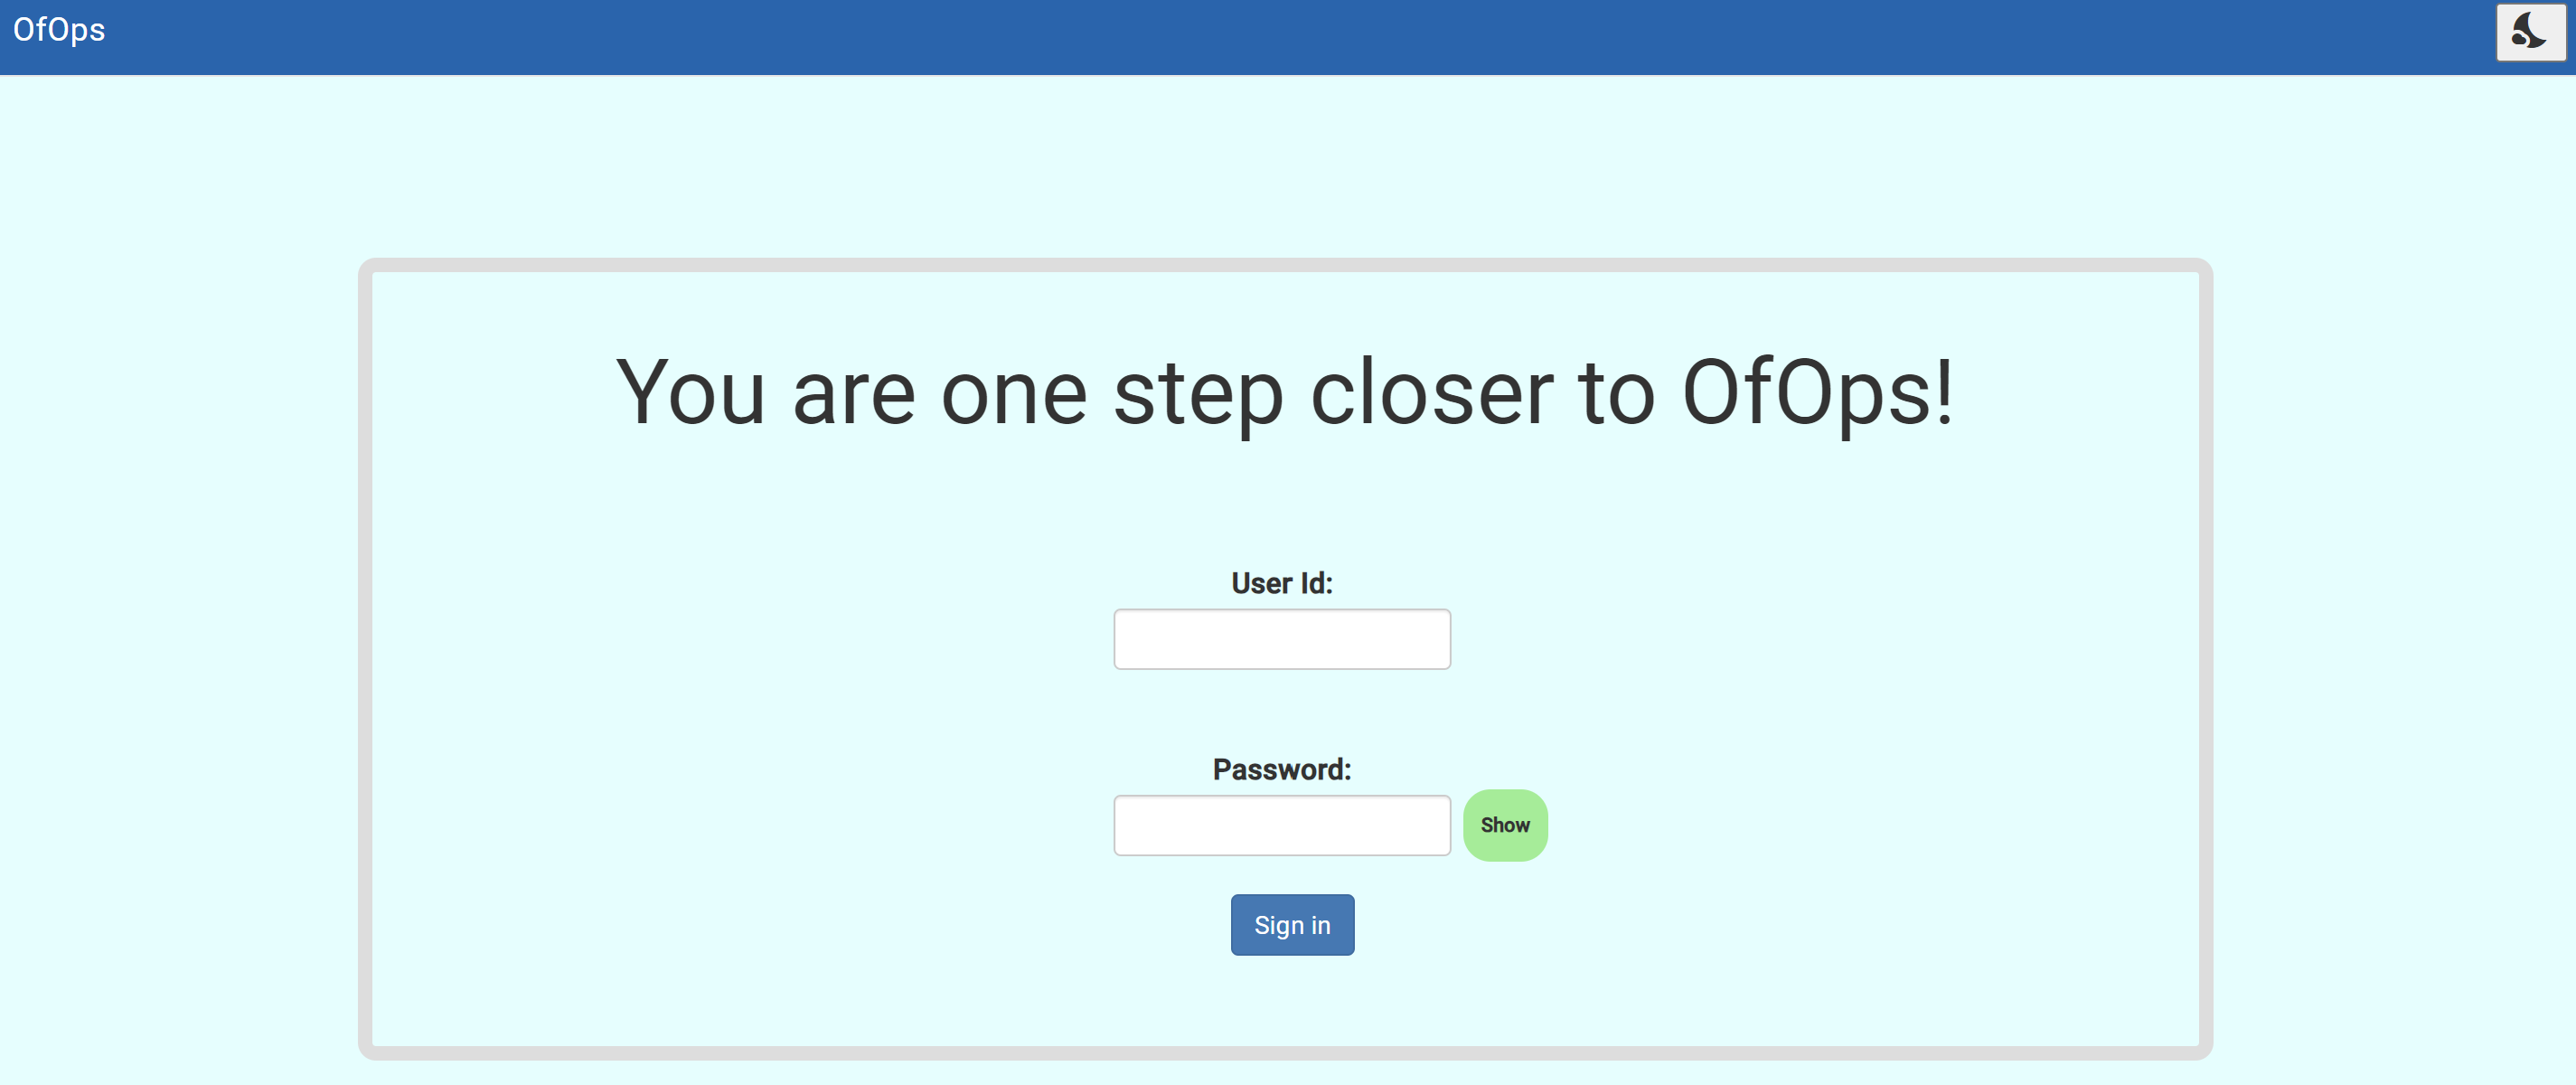
\includegraphics[width=0.9\linewidth]{images/signin.png}
    \caption{Sign in}
    \label{fig:signin}
\end{figure}

\newpage

De asemenea, după logarea în aplicațtie, utilizatorul are posbilitatea de logout.

\begin{figure}[!htb]
    \centering
    
\includegraphics[width=0.9\linewidth]{images/logout.png}
    \caption{Logout}
    \label{fig:logout}
\end{figure}

\section{Rezervarea unui loc}

Rezervarea unui loc este principala funcționalitate a aplicației. Aceasta începe prin apăsarea butonul de \textbf{Start} din pagina principală după ce utilizatorul s-a autentificat sau apăsând pe butonul \textbf{Maps}. Ulterior, user-ul va fi redirecționat către fereastra din care poate alege una dintre hărțile din dropdown. 

\newpage

\begin{figure}[!htb]
    \centering
    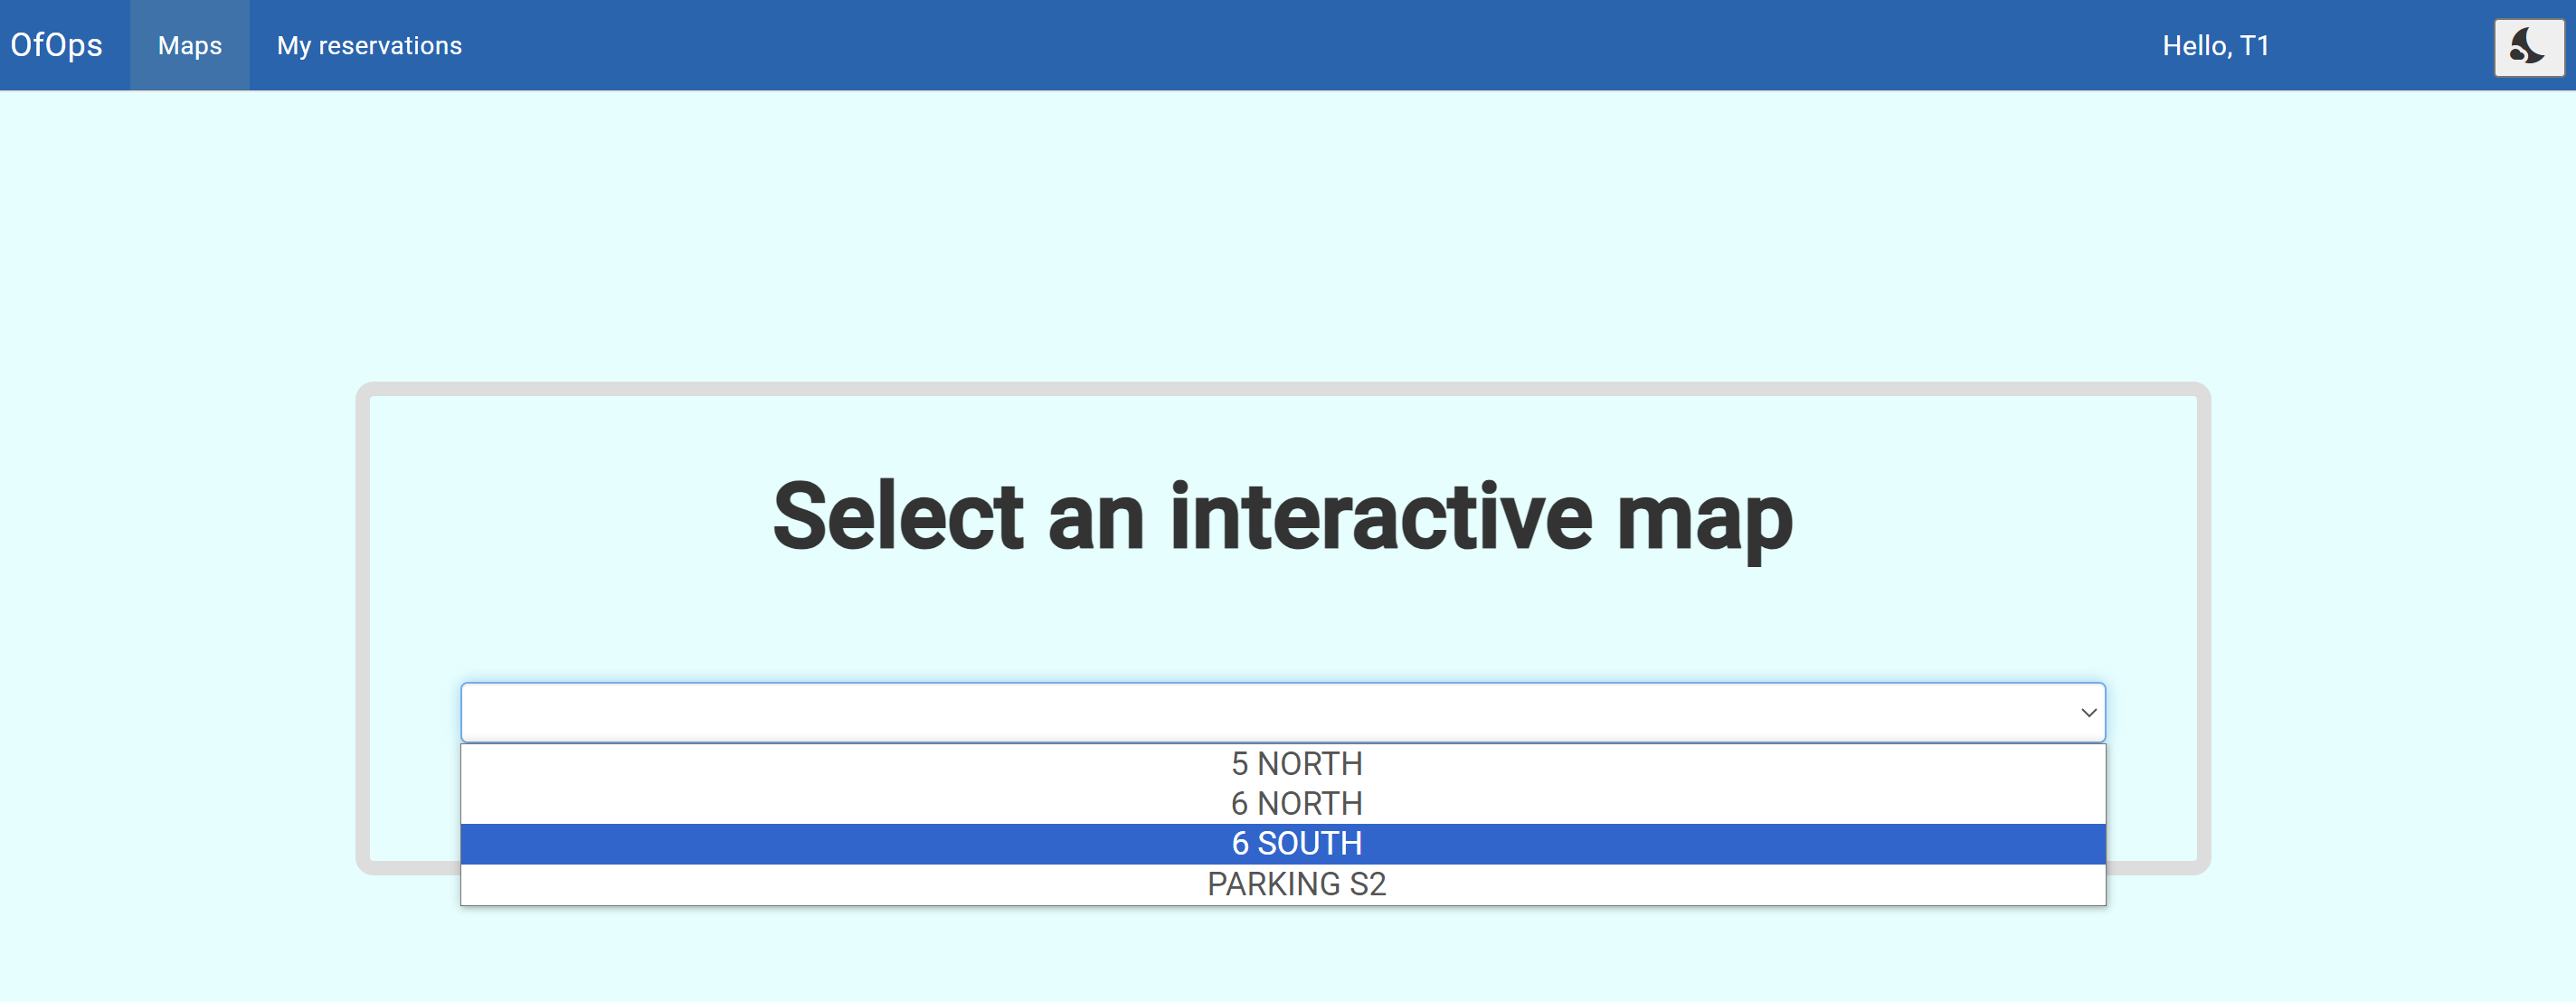
\includegraphics[width=0.9\linewidth]{images/harti.png}
    \caption{Hărțile disponibile}
    \label{fig:harti}
\end{figure}

Odată selectată o hartă, va trebui aleasă ziua în care se dorește a fi rezervarea. Din calendarul apărut, utilizatorul nu poate alege zilele de weekend sau zilele din trecut, întrucât reținerea locurilor în trecut sau în zilele de sâmbătă și duminică este inutilă.  

\begin{figure}[!htb]
    \centering
    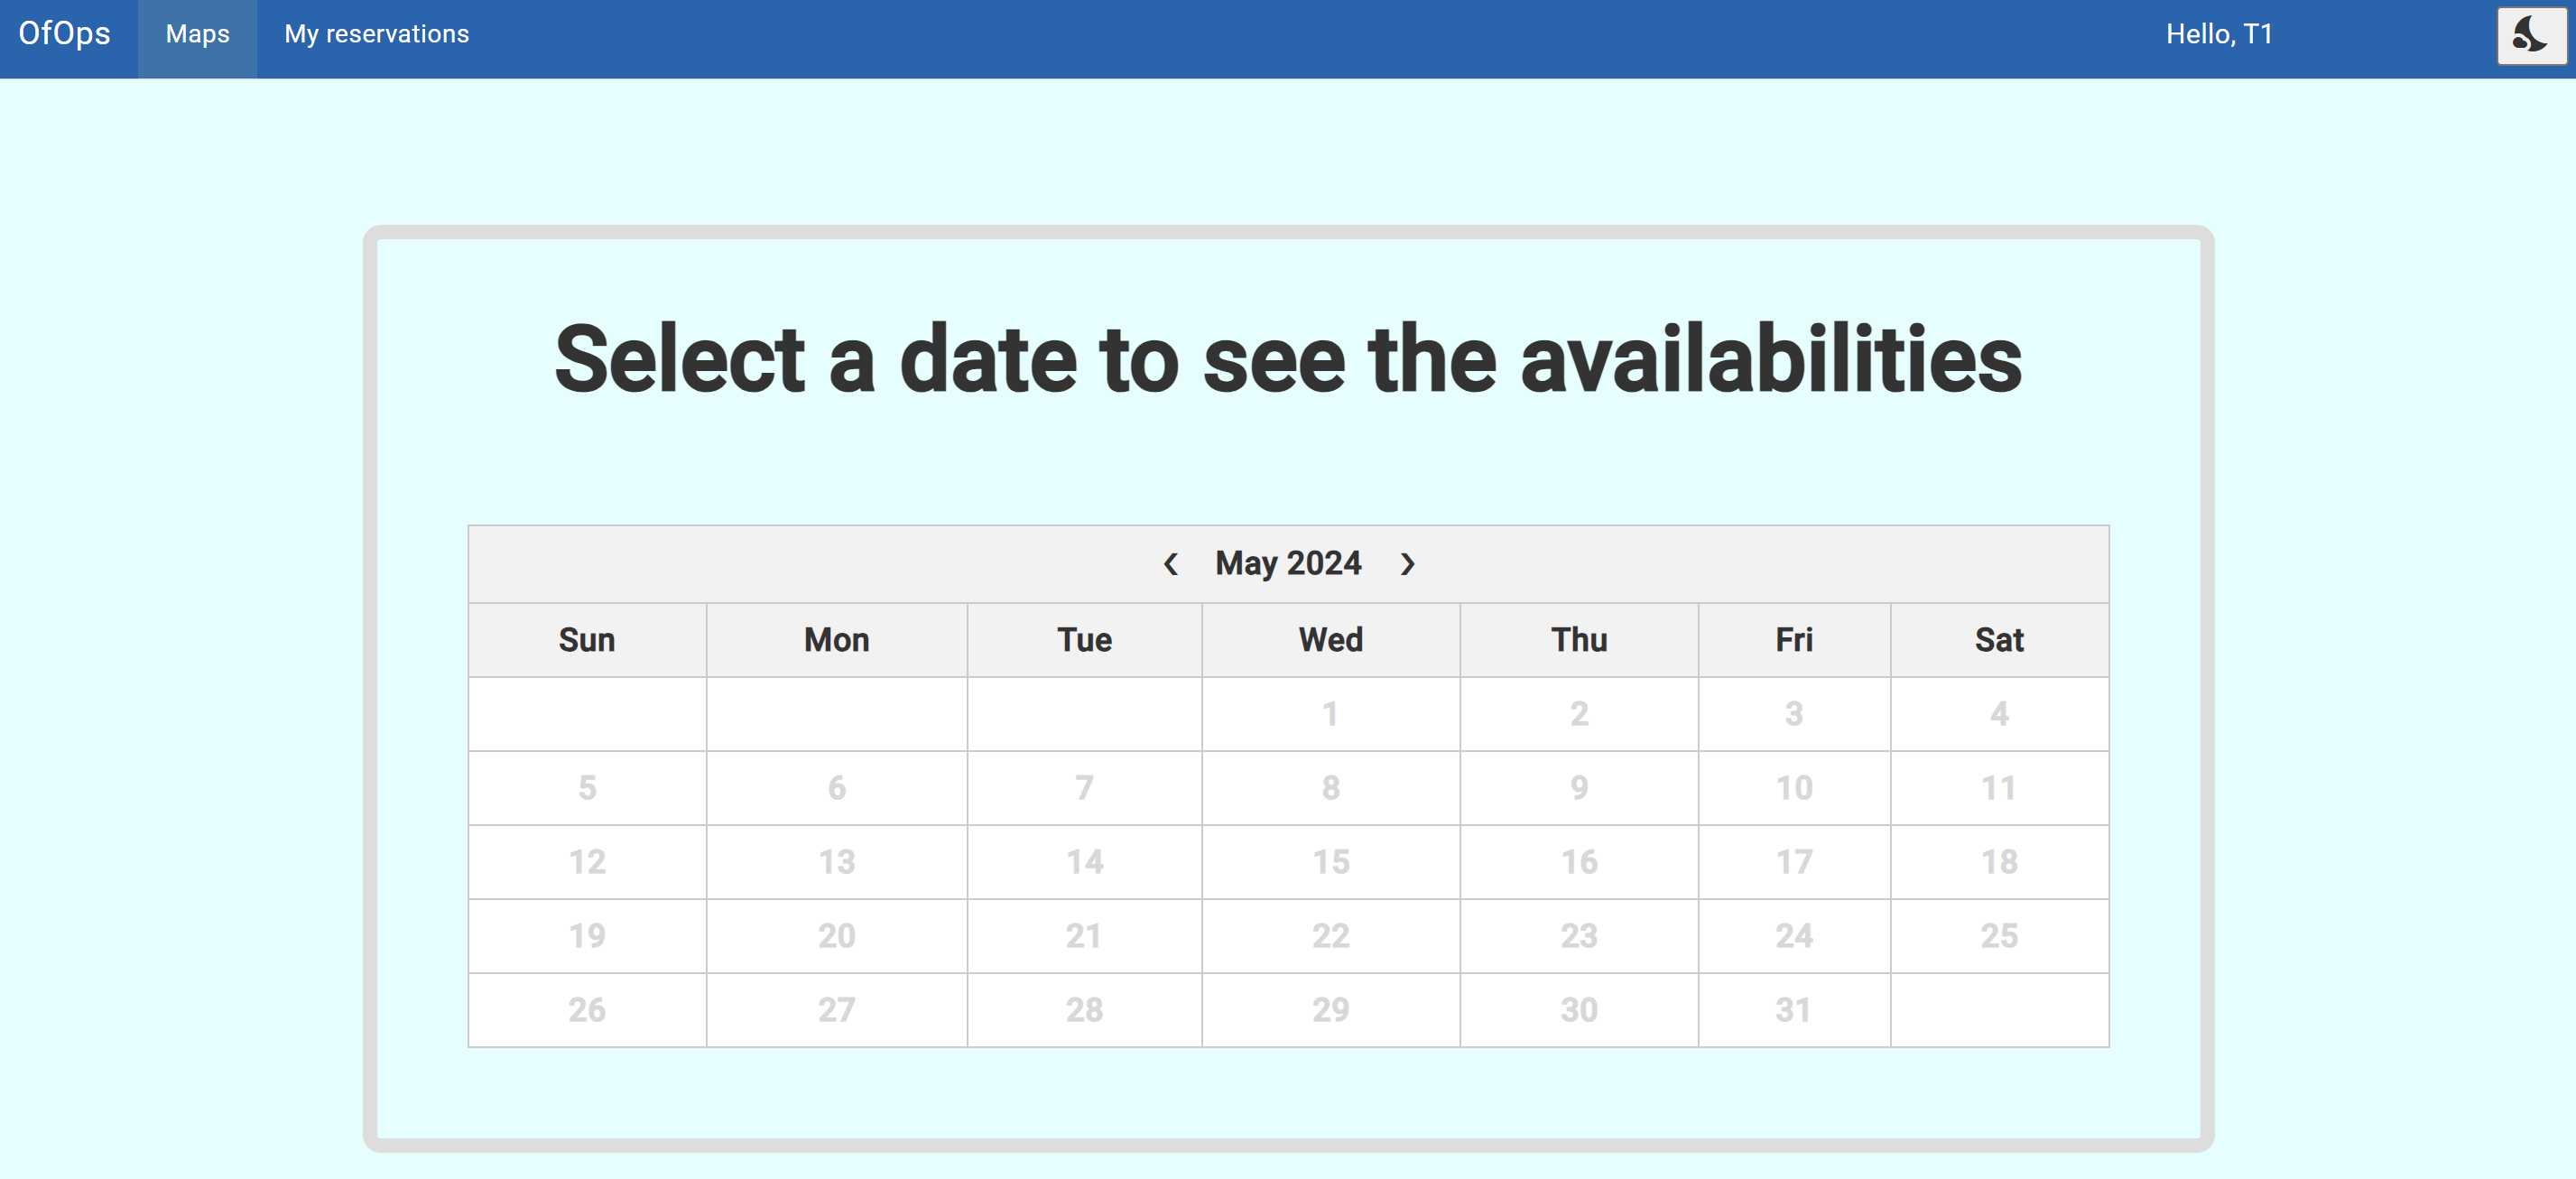
\includegraphics[width=0.9\linewidth]{images/calendar vechi.png}
    \caption{Calendarul cu luna mai}
    \label{fig:calendarvechi}
\end{figure}

Selectarea datei este însoțită de un popup pentru exprimarea dorinței de a rezerva în acea zi pe care utilizatorul trebuie să o confirme sau nu, după preferințele sale.

\newpage

\begin{figure}[!htb]
    \centering
    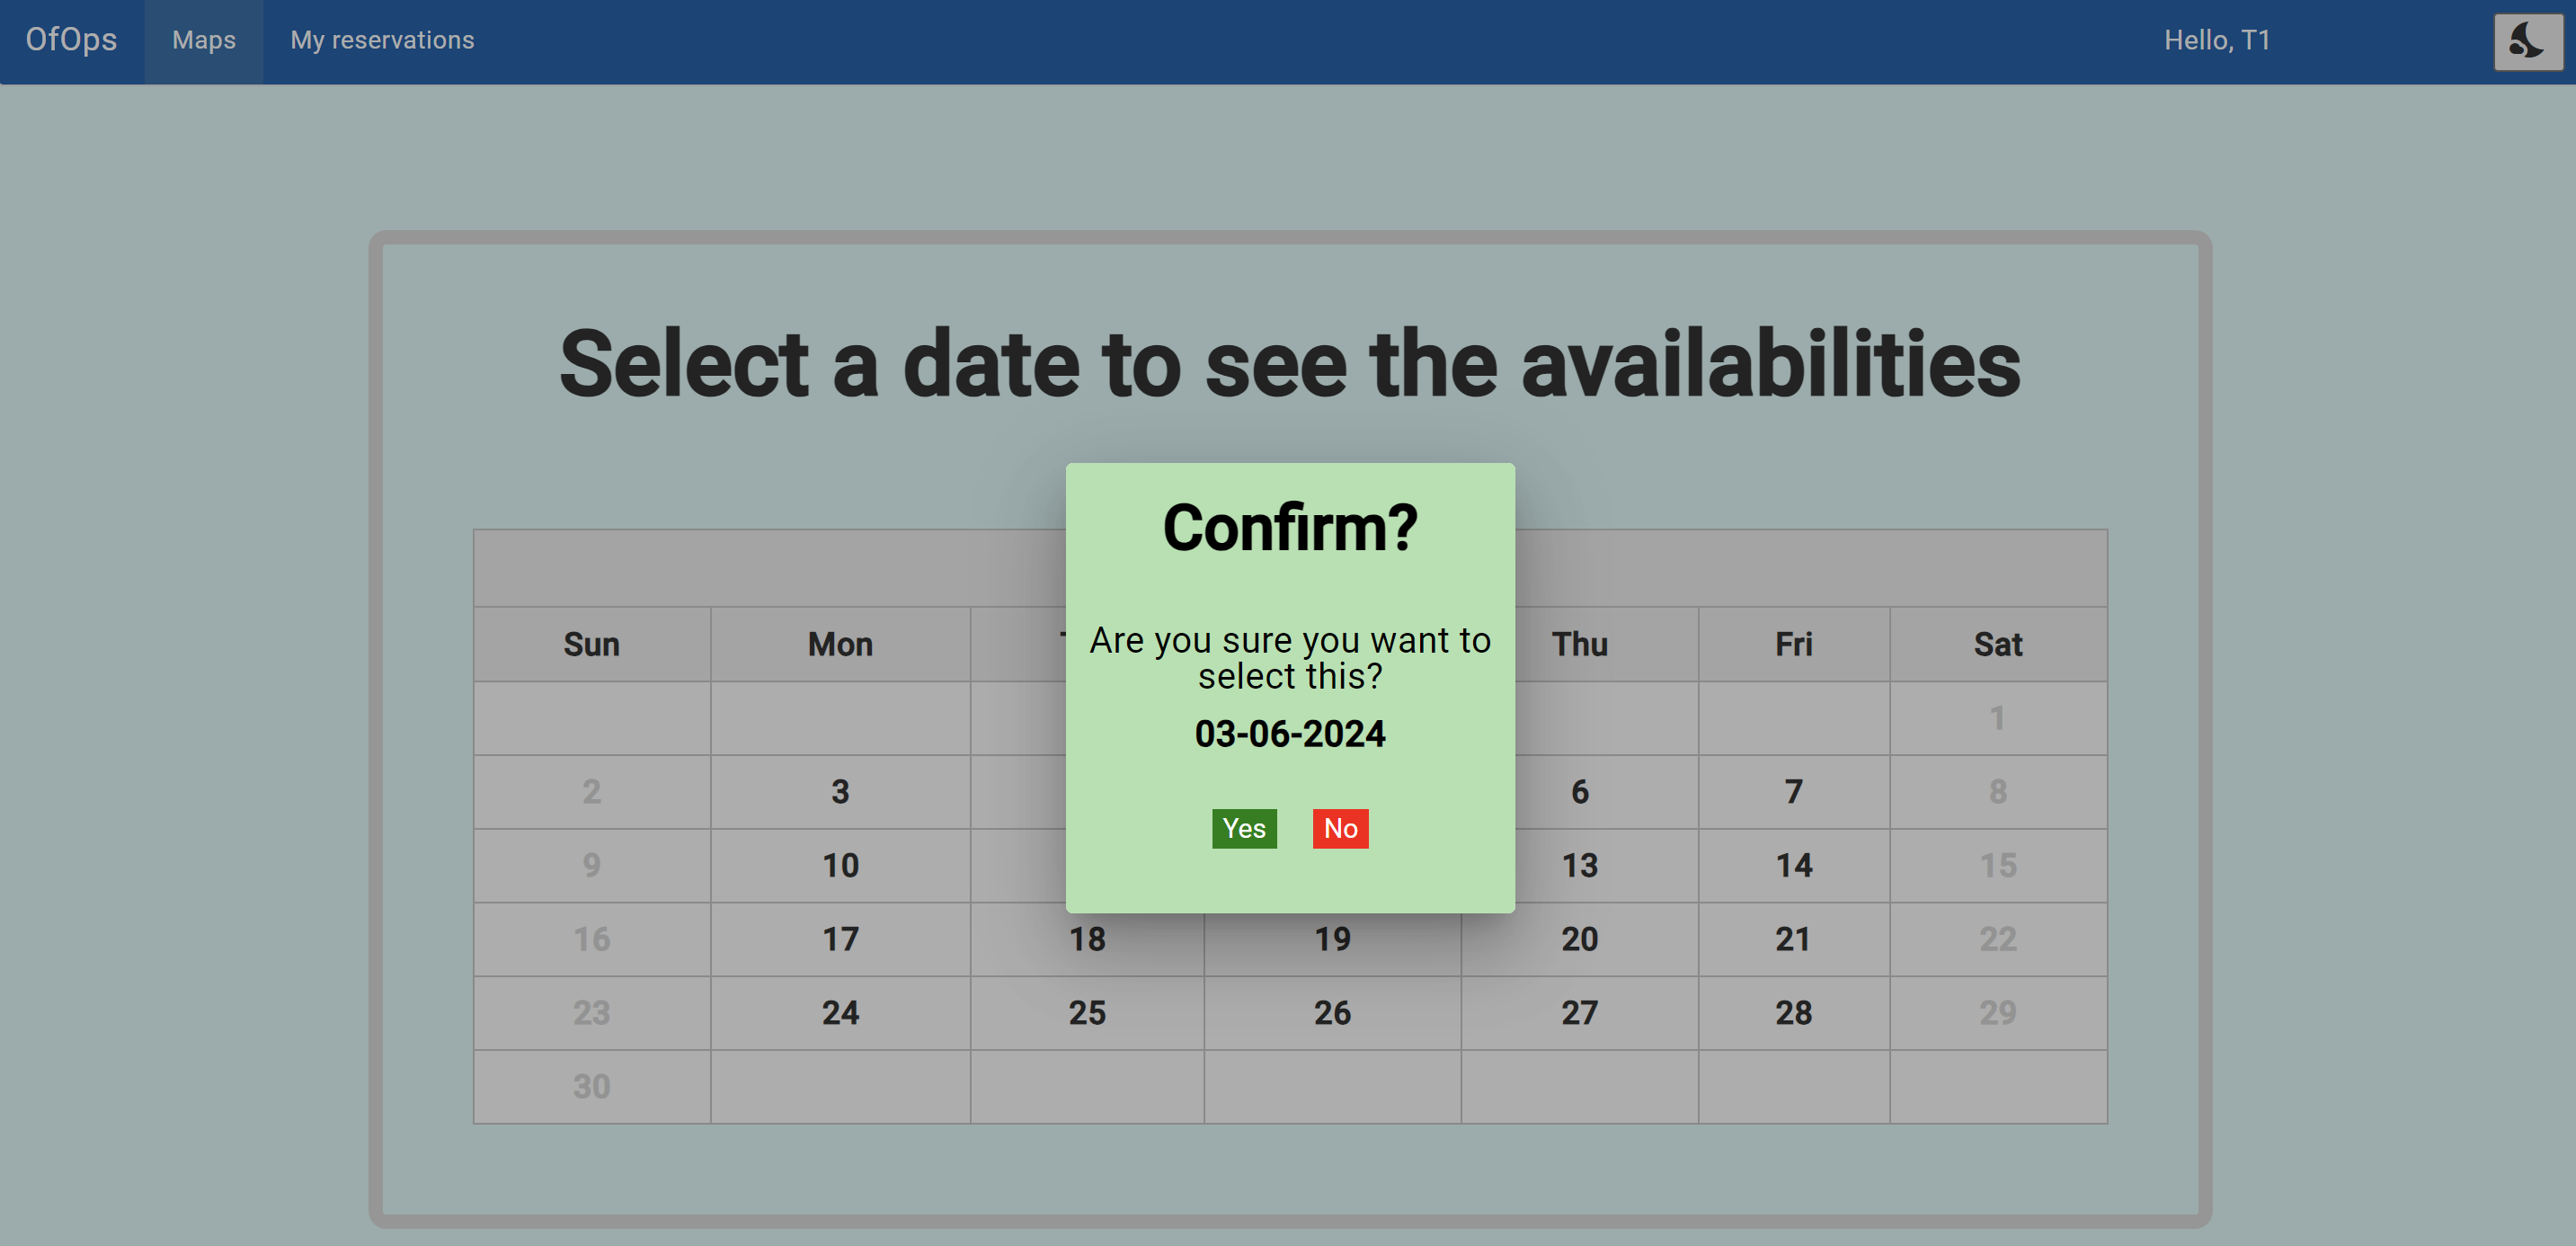
\includegraphics[width=0.9\linewidth]{images/calendar bun.png}
    \caption{Popup pentru confirmare}
    \label{fig:calendarbun}
\end{figure}

Ulterior, se va face redirecționarea către ceasul unde se va alege momentul la care utilizatorul vrea să vadă disponibilitățile. Mai întâi se selectează ora. Click-ul pe ora dorită va declanșa apariția butoanelor AM-PM, iar alegerea formatului va duce la apariția minutelor. Am decis ca implementarea butoanelor să fie pentru fiecare minut, întrucât pot exista momente în care se dorește o verificare a locurilor libere într-un moment actual, în care ora nu este fixă. Alegerea completă a timpului duce la apariția butonului de \textbf{Choose time}, însoțit de rezultatul selectării timpului.

\begin{figure}[!htb]
    \centering
    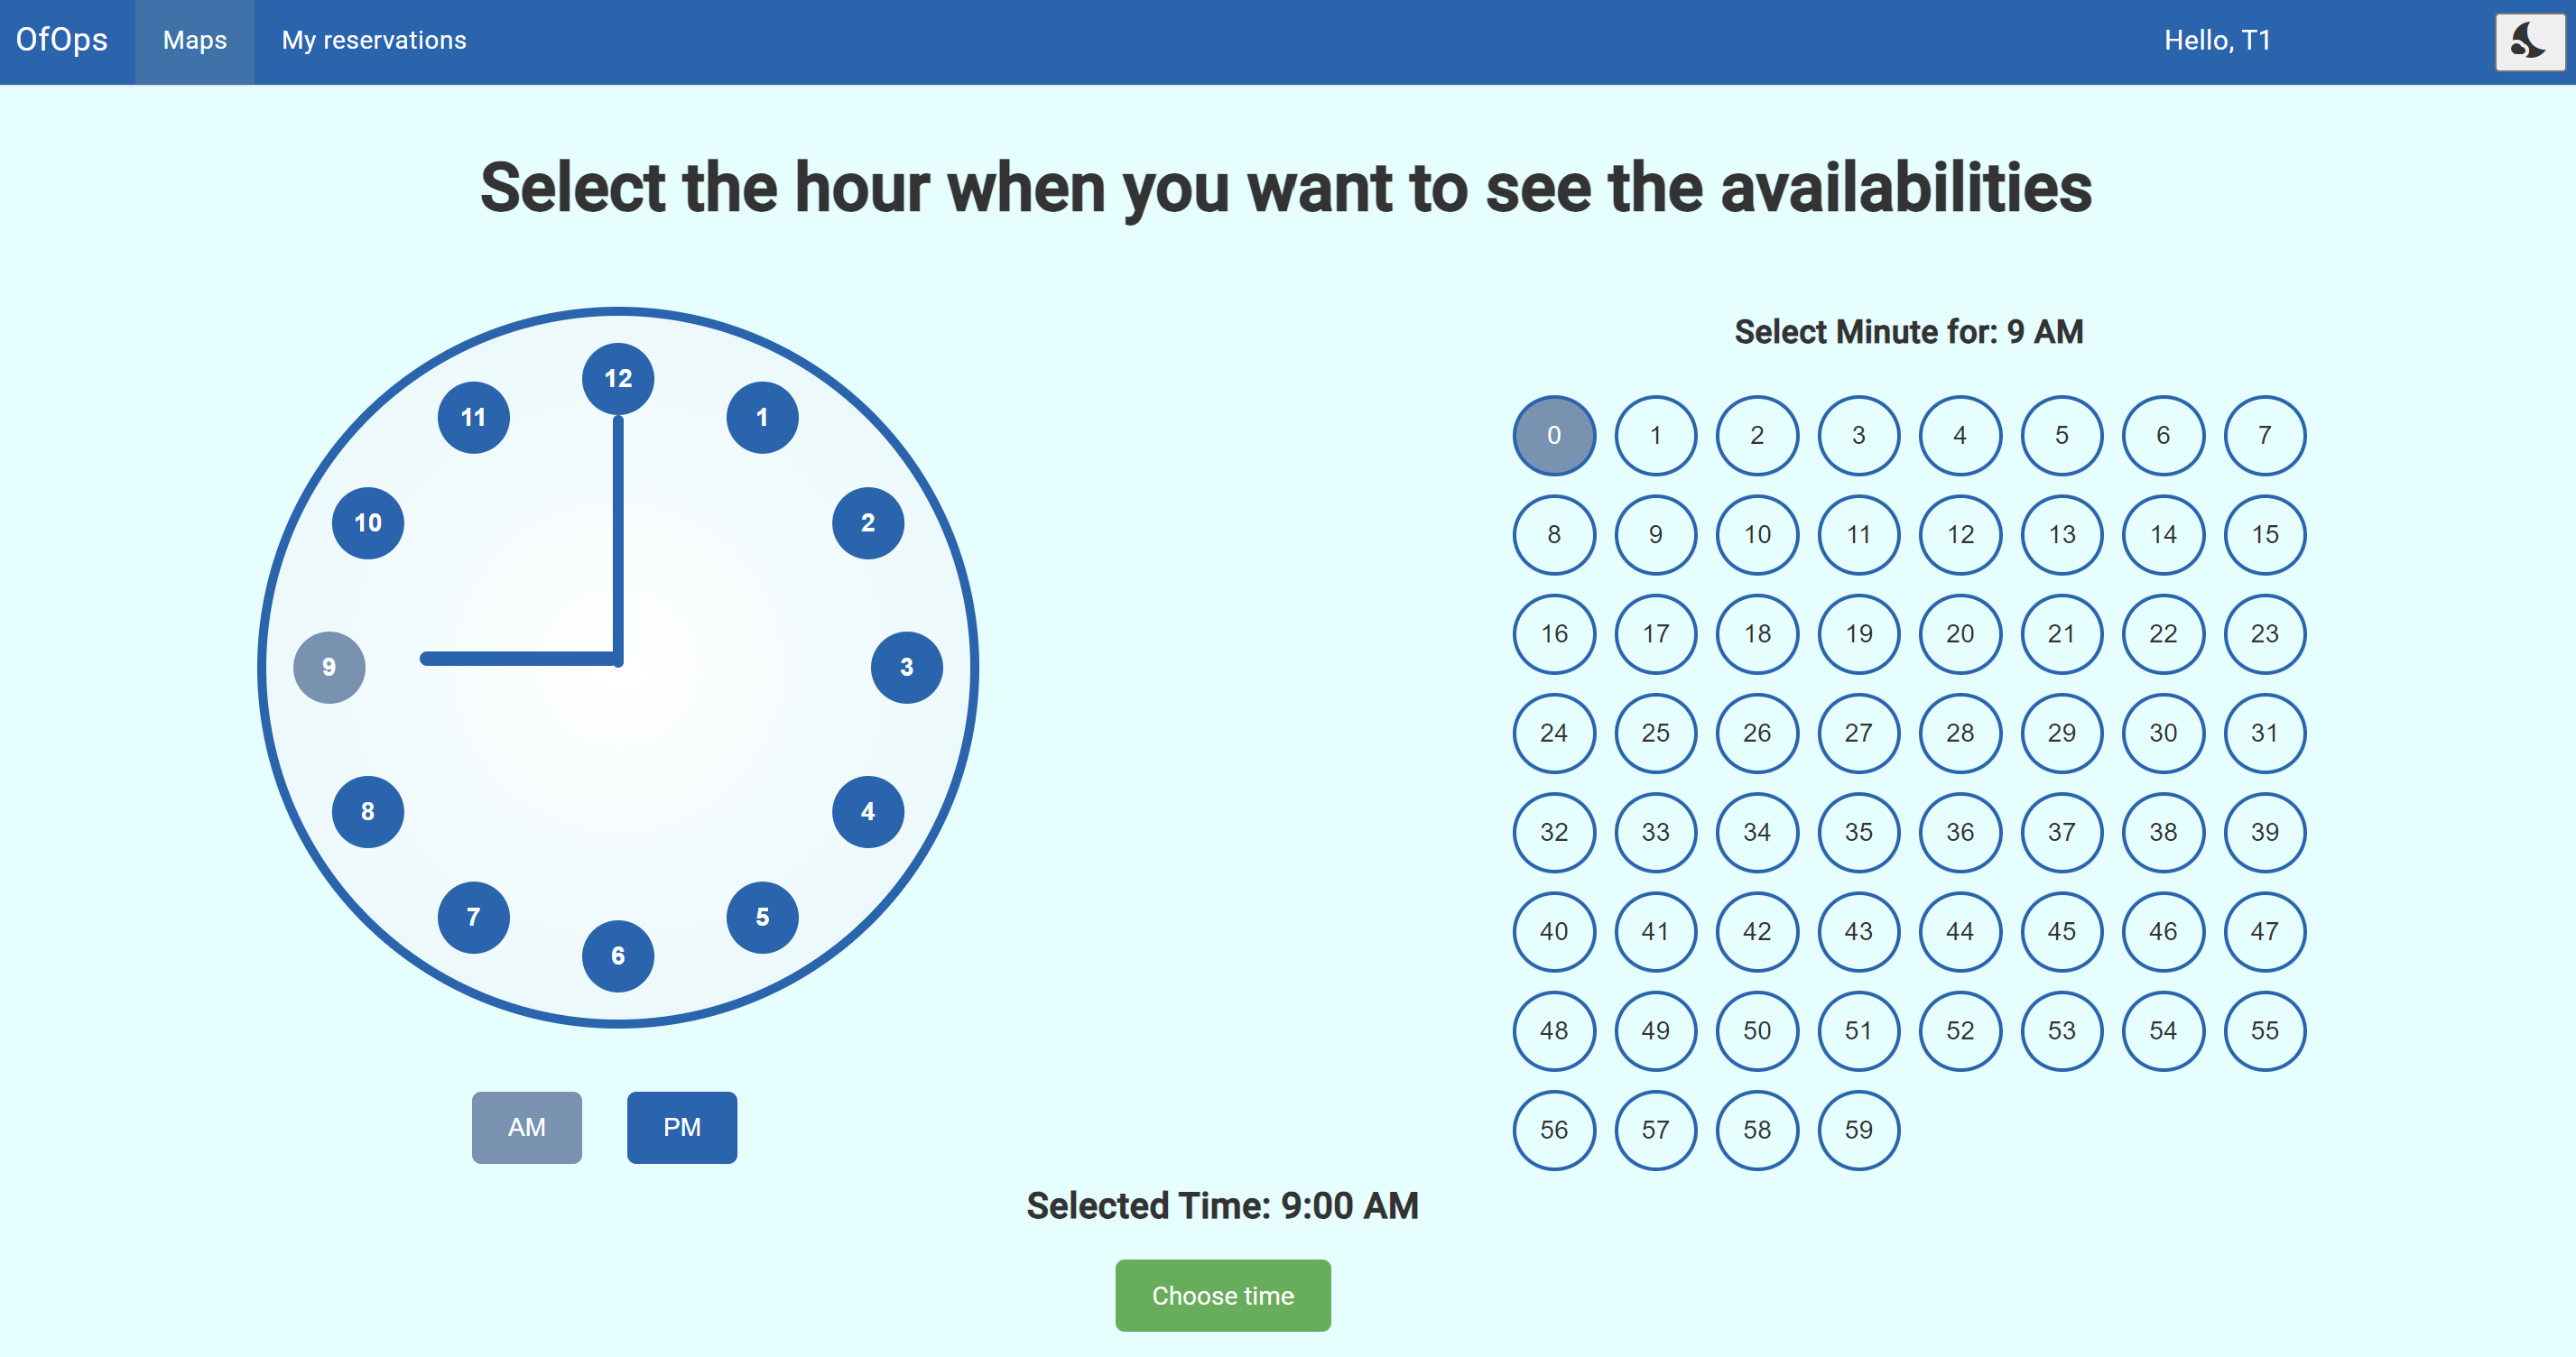
\includegraphics[width=0.9\linewidth]{images/timp.png}
    \caption{Selectarea corectă a timpului}
    \label{fig:timp}
\end{figure}

Toți acești pași ne conduc către harta interactivă pentru alegerea unui birou sau a unui loc de parcare în funcție de preferință.

\newpage

\begin{figure}[!htb]
    \centering
    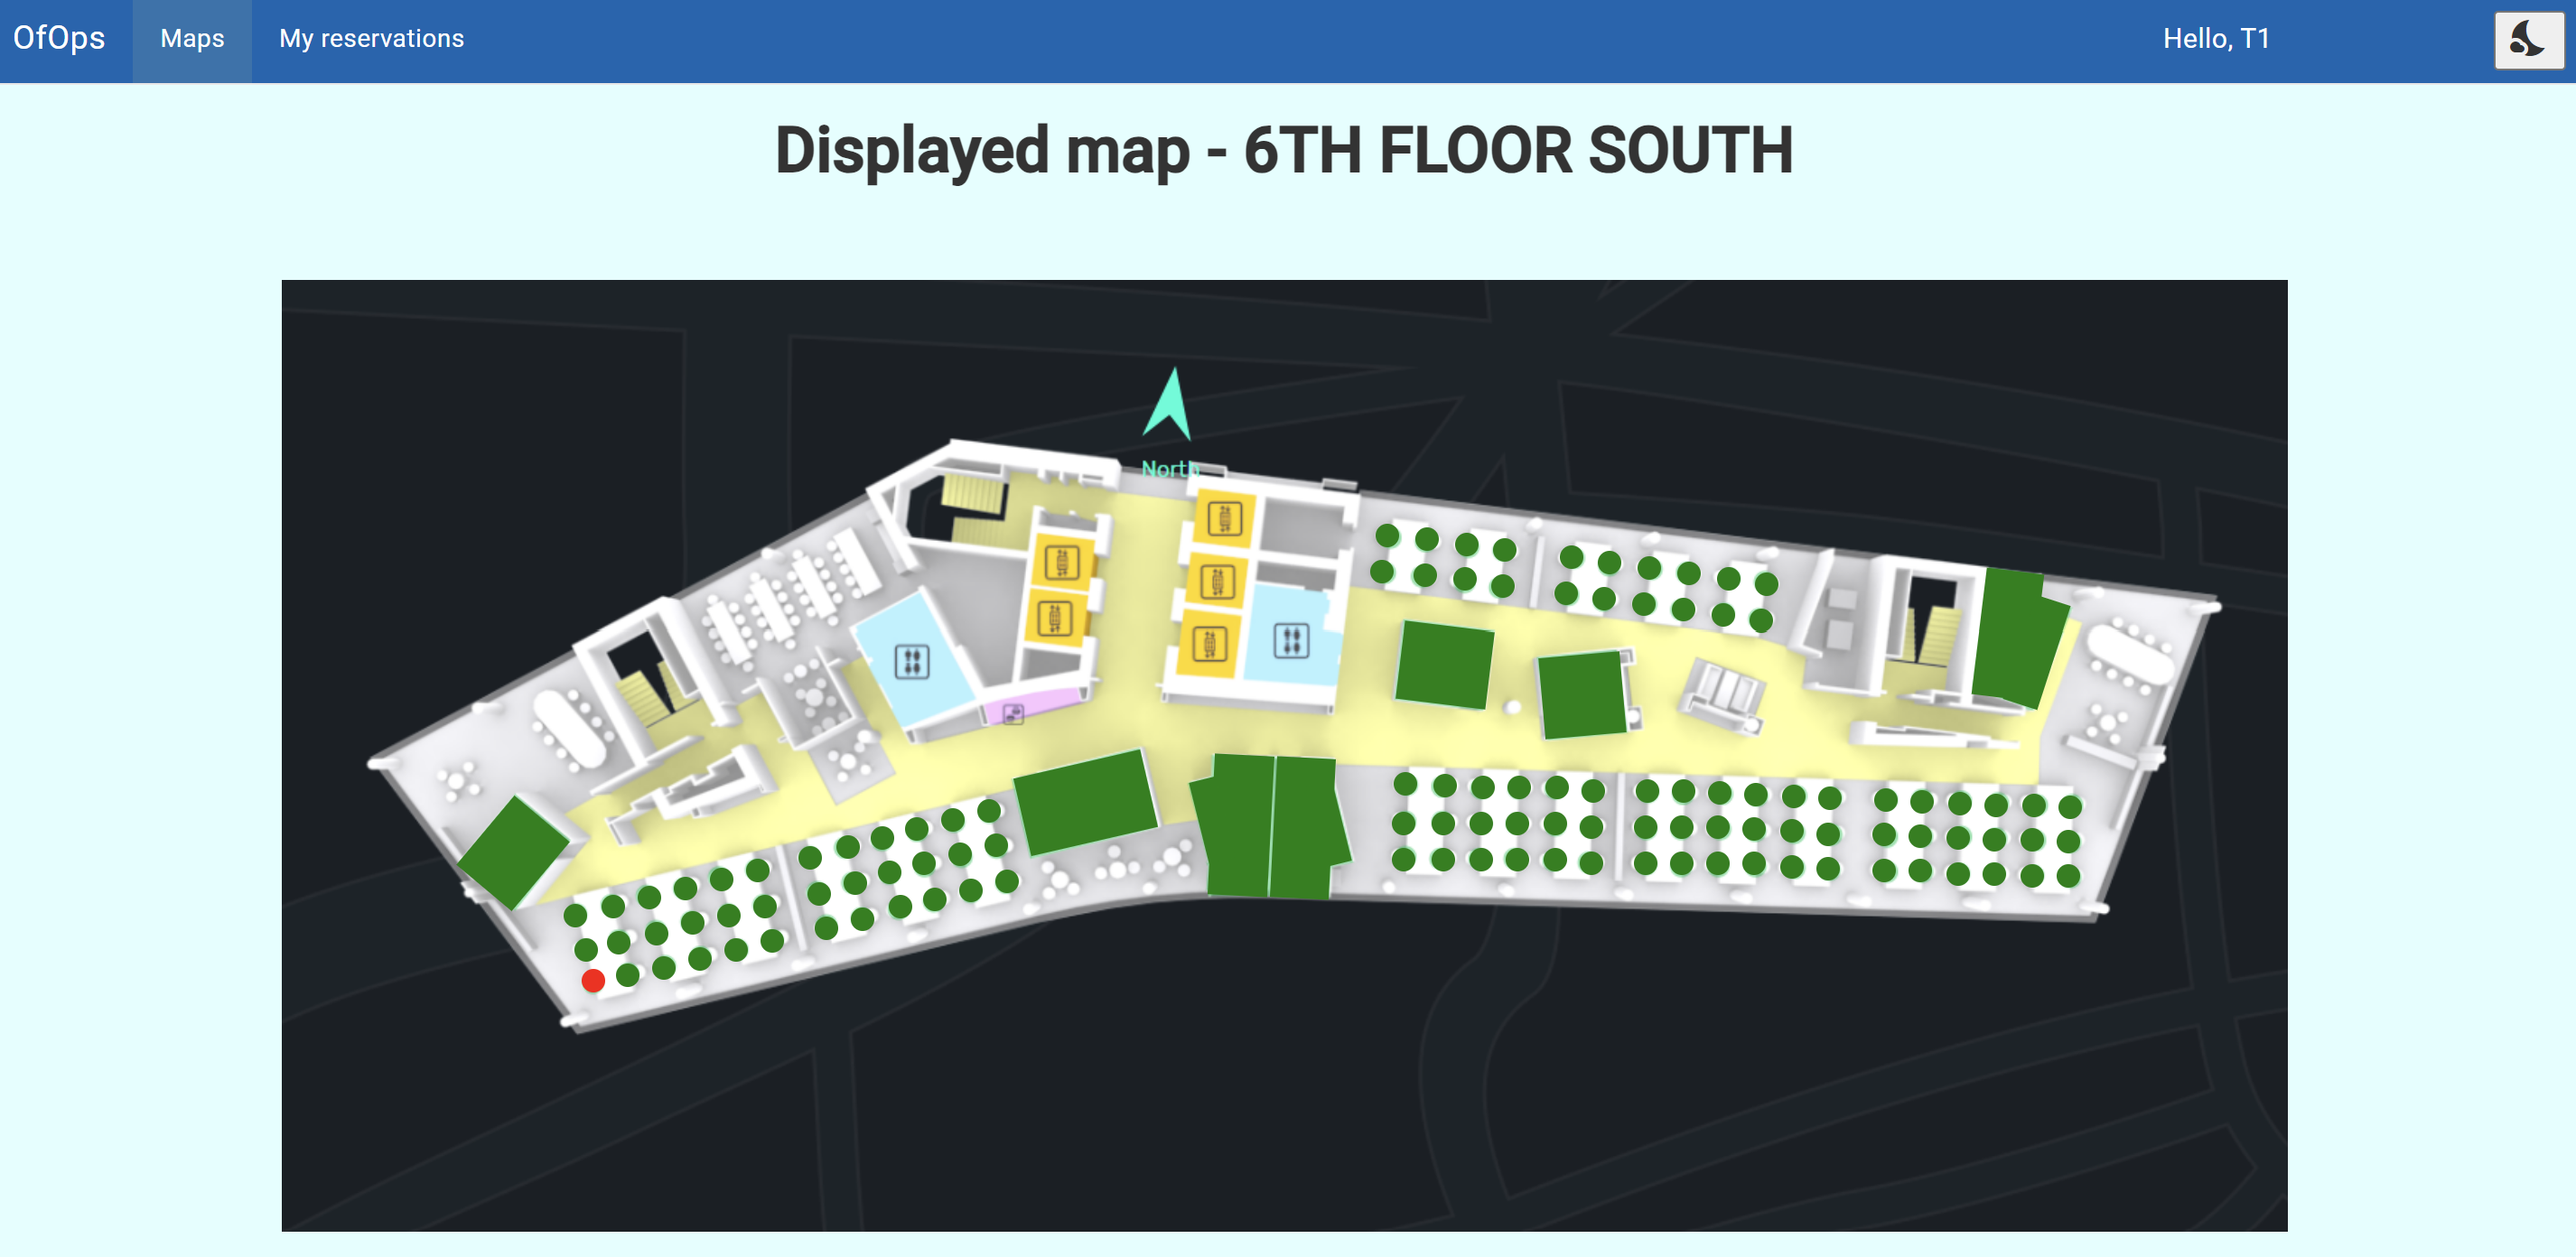
\includegraphics[width=0.9\linewidth]{images/hartaint.png}
    \caption{Harta interactivă pentru etajul 6 SUD}
    \label{fig:hartaint}
\end{figure}

Printr-o privire foarte rapidă asupra hărții, se poate remarca că o bulină (reprezentând un birou) este roșie. Aceasta semnifică faptul că biroul este rezervat în momentul în care utilizatorul a ales să verifice disponibilitatea. Bulinele verzi indică faptul că nu există o rezervare la ora dorită pentru birourile respective. Fiind harta interactivă, alegerea unui loc se face apăsând direct pe biroul respectiv.

\begin{figure}[!htb]
    \centering
    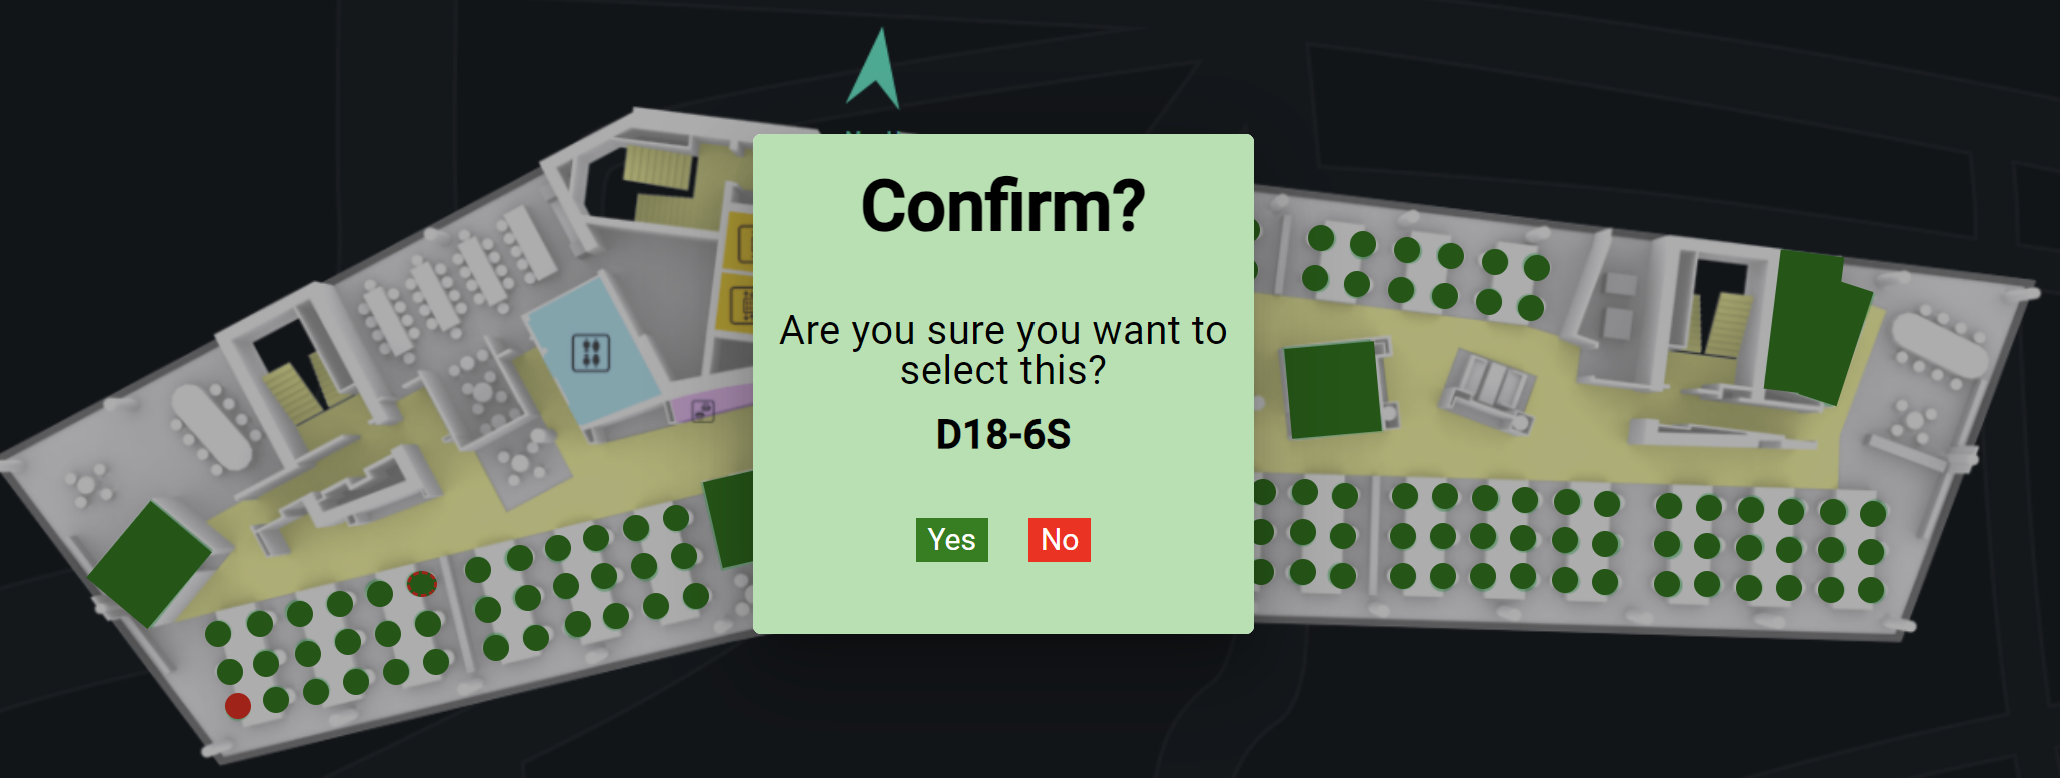
\includegraphics[width=0.9\linewidth]{images/rezerv.png}
    \caption{Confirmare loc}
    \label{fig:rezerv}
\end{figure}

Înainte de rezervarea propriu-zisă, utilizatorului îi va apărea un popup de confirmare pentru selectarea locului. Se poate observa, de asemenea, că locul selectat este înconjurat de o linie punctată, astfel încât user-ul să vadă precis ce loc dorește să rezerze înainte de a apăsa butonul \textbf{Yes}.

În cazul în care există o rezervare viitoare pentru locul selectat, utilizatorul va primi o notificare în acest sens. Dacă utilizatorul alege să selecteze acest birou, rezervarea sa trebuie făcută în cunoștință de cauză sau poate alege alt loc.

\newpage

\begin{figure}[!htb]
    \centering
    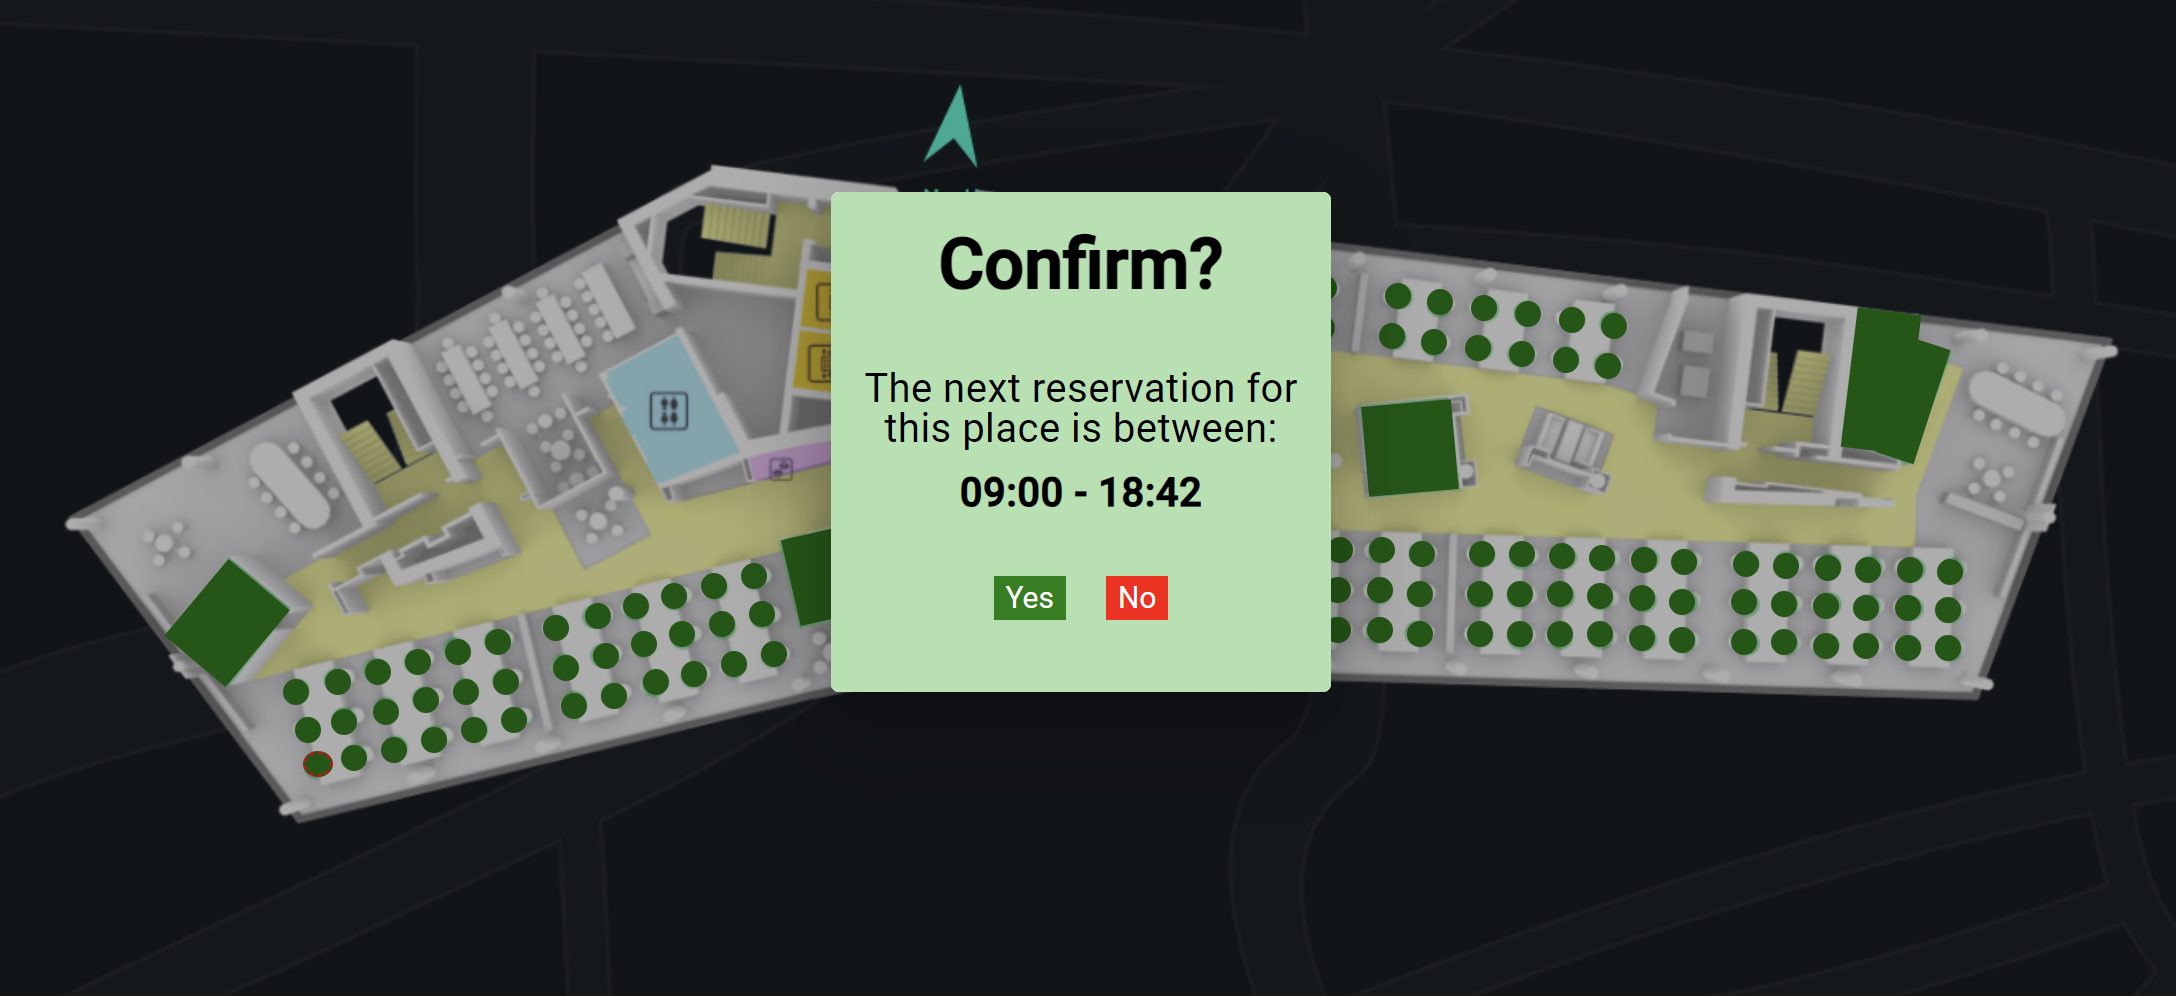
\includegraphics[width=0.9\linewidth]{images/notif.png}
    \caption{Notificare rezervare următoare}
    \label{fig:notif }
\end{figure}

Rezervarea unui birou se realizează în pagina dedicată acesteia. Câmpurile de completat sunt cele de \textbf{Start Time}, \textbf{End Time} și \textbf{Event}. \textbf{Selected Date} nu se poate modifica, având rolul de a-i aminti user-ului data selectată. Dacă acesta nu mai dorește o rezervare în ziua selectată, trebuie să reia întreg procesul de rezervare. Butonul de \textbf{Submit} nu se va activa până când datele nu sunt completate, evitând, astfel, introducerea în baza de date a unor câmpuri goale. Dacă totul este în regulă, se poate efectua rezervarea, iar utilizatorul va fi redirecționat către pagina de \textbf{My reservations} care va fi detaliată într-un subcapitol următor.

\begin{figure}[!htb]
    \centering
    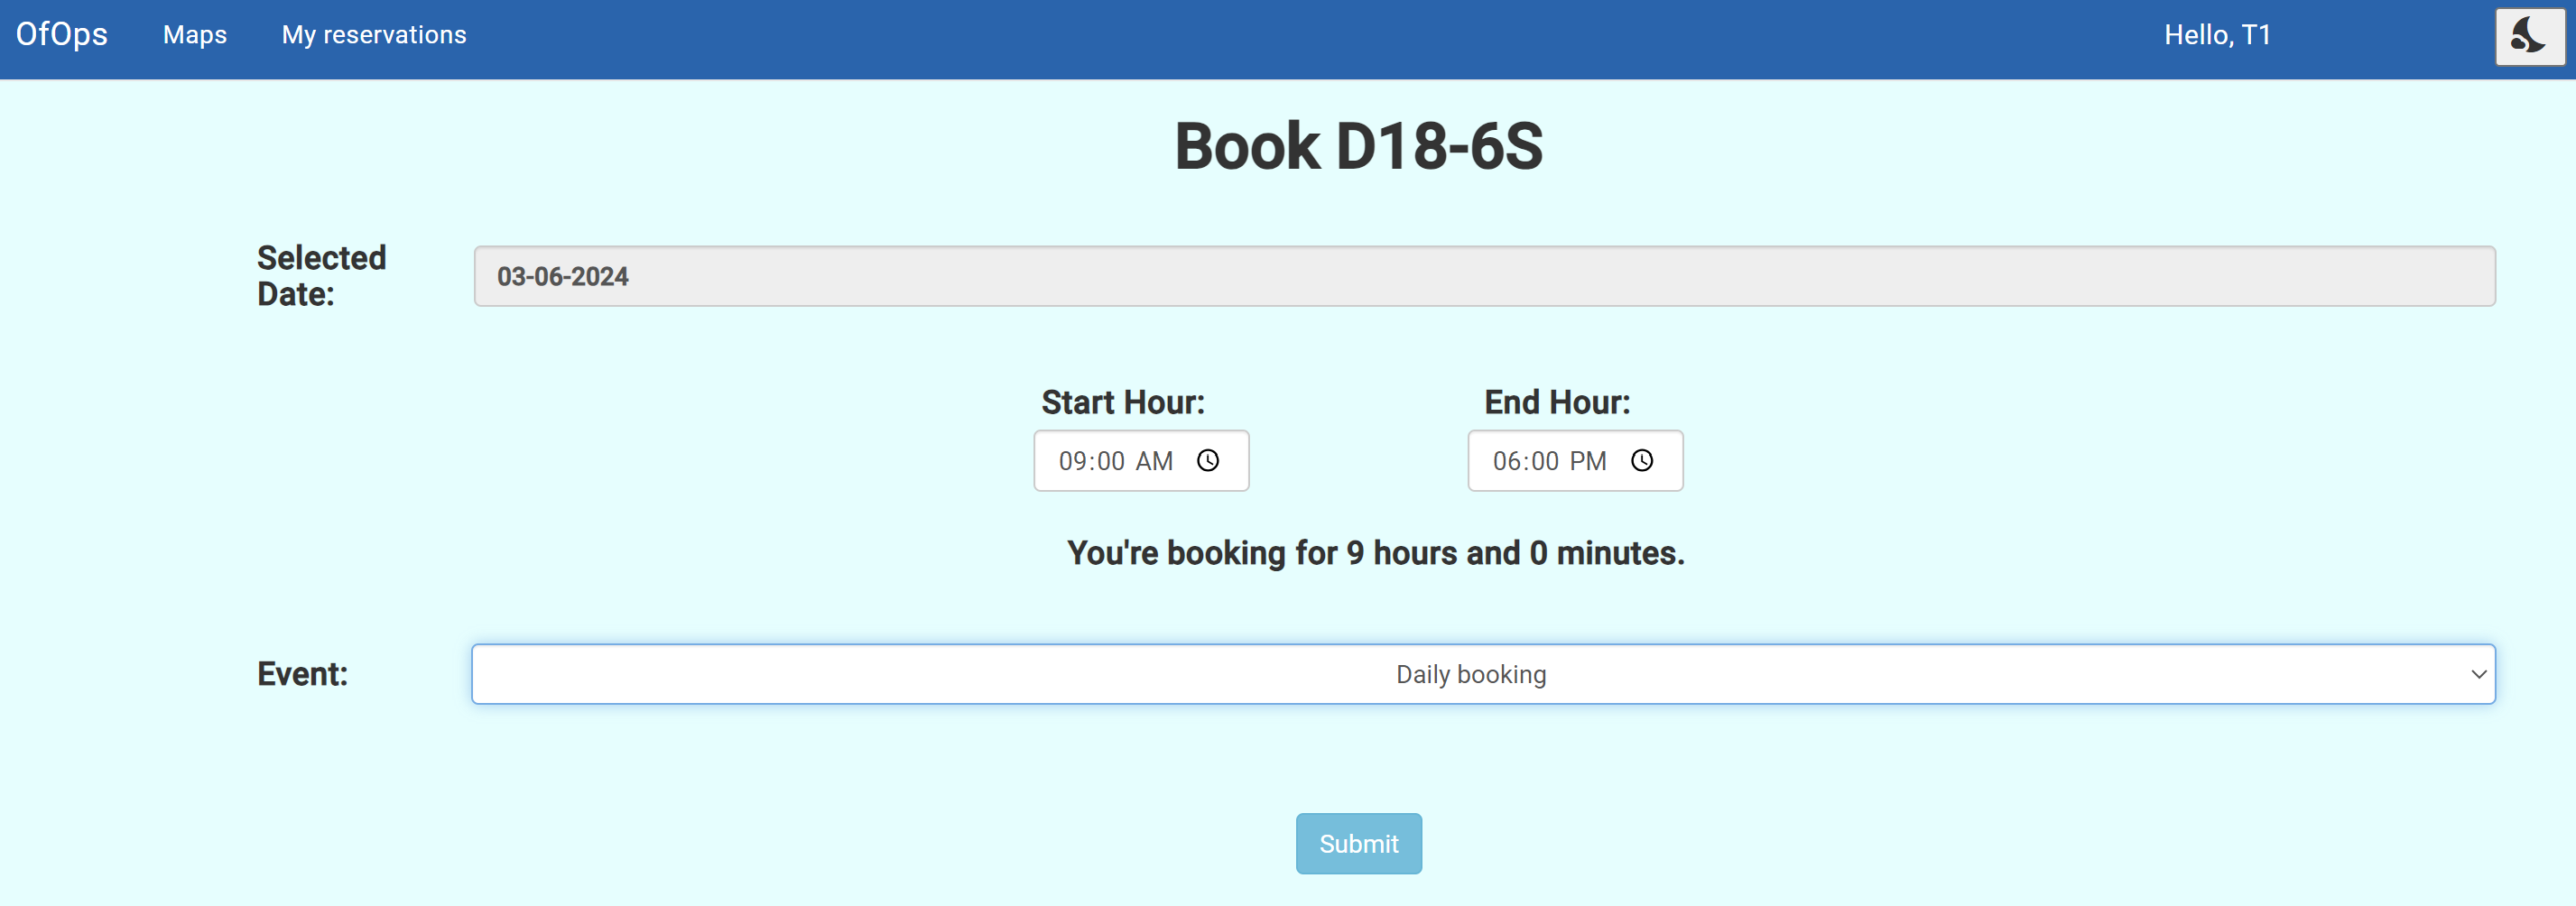
\includegraphics[width=0.9\linewidth]{images/rezerv corecta.png}
    \caption{Rezervare corectă}
    \label{fig:rezerv corecta }
\end{figure}

Există posibilitatea ca rezervarea pe care dorește să o facă utilizatorul în momentul curent să se suprapună cu o altă rezervare deja făcută pentru același loc. OfOps nu va permite întâmplarea acestui lucru! Încercarea de a rezerva totuși va duce la apariția unui mesaj care va indica ora următoarei rezervări, iar butonul de \textbf{Submit} se va dezactiva.

\begin{figure}[!htb]
    \centering
    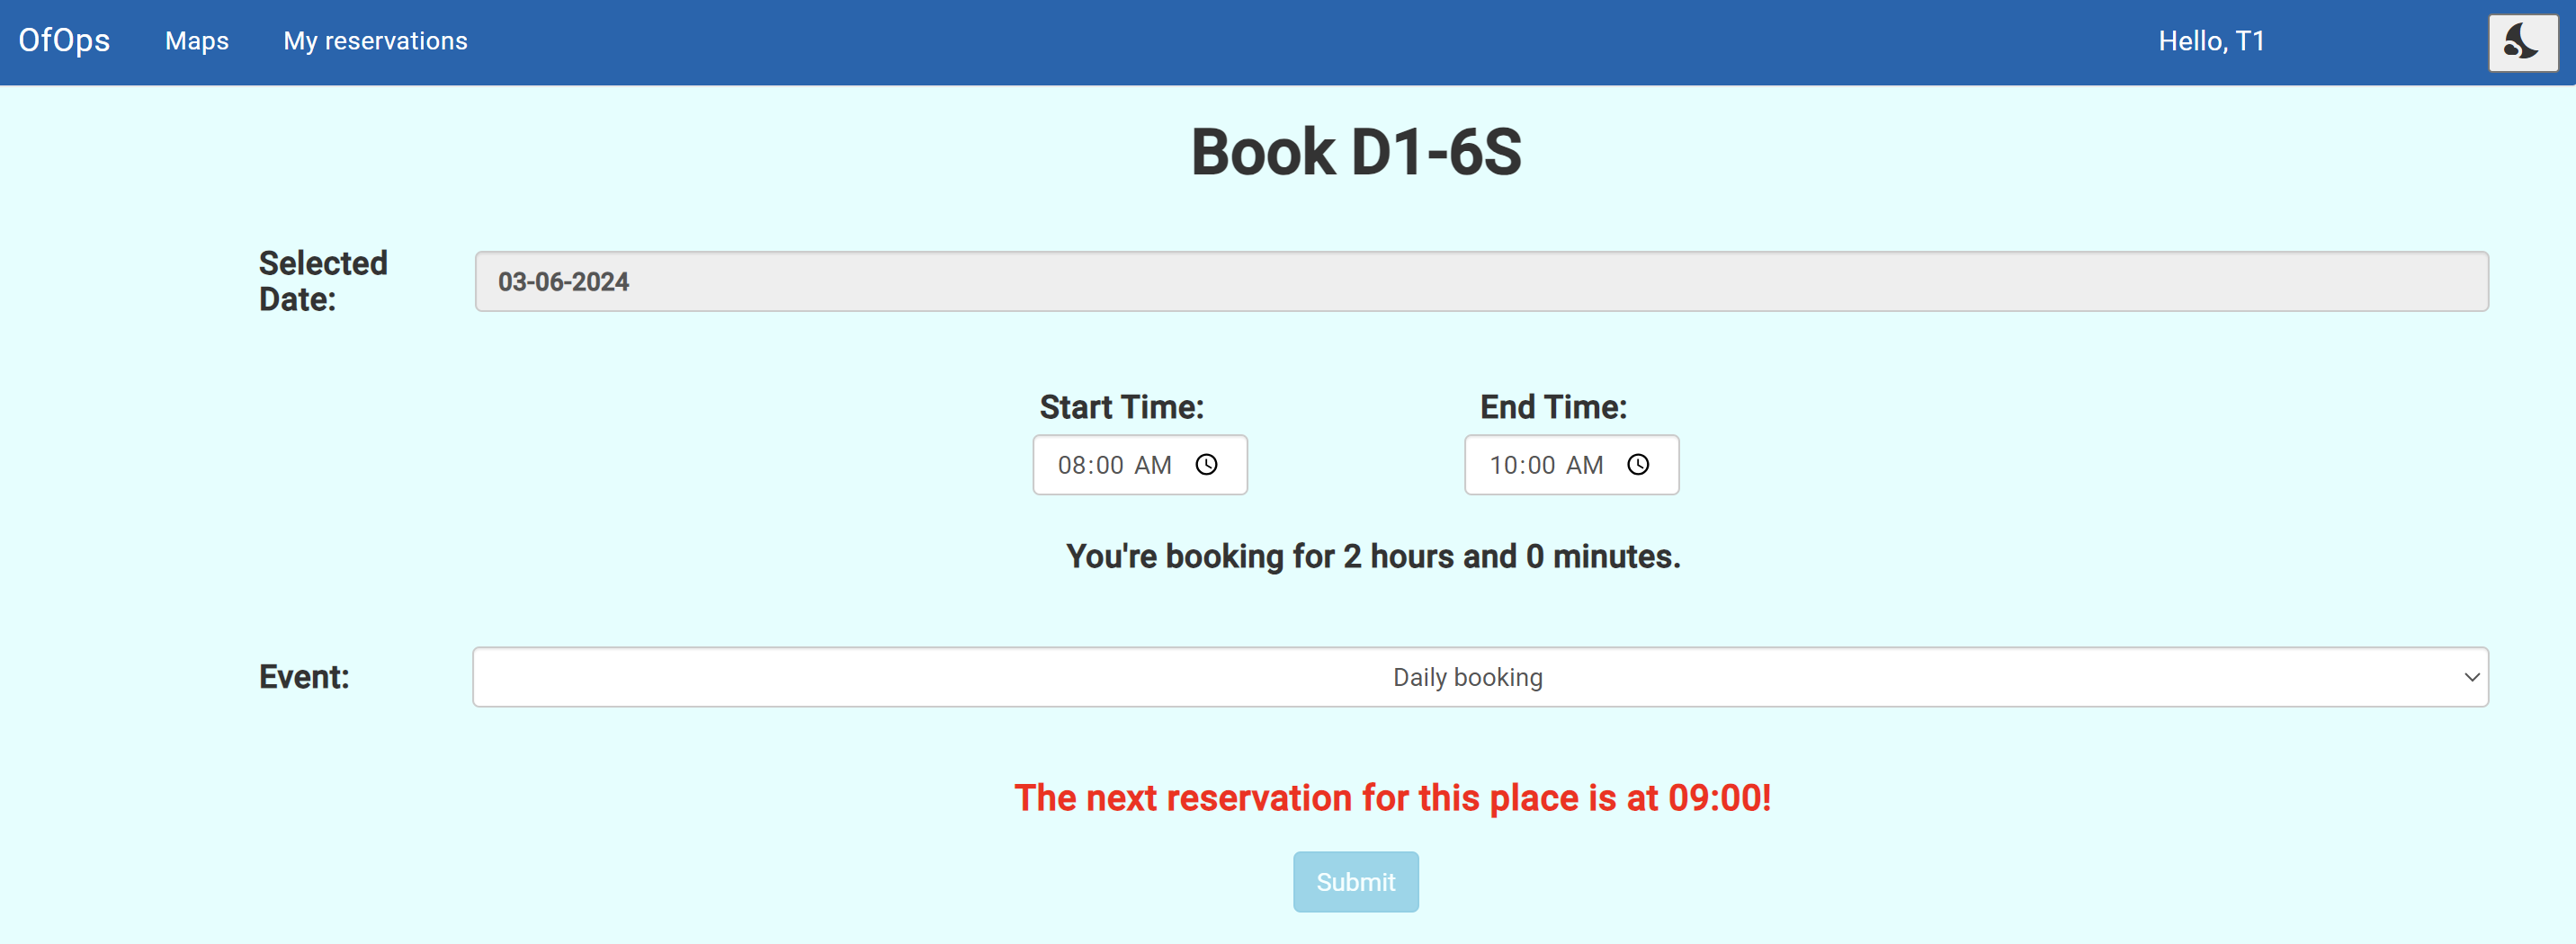
\includegraphics[width=0.9\linewidth]{images/rezerv incorect.png}
    \caption{Rezervare incorectă}
    \label{fig:rezerv incorect}
\end{figure}

\section{Rezervarea unei săli de ședință}

Rezervarea unei săli de ședință urmează același curs ca rezervarea unui birou sau al unui loc de parcare, însă are ceva în plus față de celelalte. Atunci când un utilizator încearcă să rezerve o sală de ședință, dacă intervalul dorit se suprapune chiar și un minut cu o altă rezervare, user-ul va primi ca alertă o propunere de sală liberă în perioada dorită. Acest lucru scoate OfOps în evidență, întrucât are dispune de o metodă care eficientizează programarea sălilor de ședință. Acest algoritm implică obținerea tuturor sălilor de ședință și calcularea unui scor de disponibilitate după care sălile sunt sortate. Metoda de calculare a punctajului de disponibilitate se rezumă la numărul de rezervări existente care se suprapun cu intervalul de timp specificat. Scorul se va incrementa doar dacă există suprapunere între rezervări, sortarea crescătoare oferindu-ne, asfel, prima opțiune cu scorul cel mai mic. Utilizatorul poate alege varianta propusă, apăsând \textbf{OK} sau pot refuza propunerea prin apăsarea \textbf{Cancel}, fiind redirecționați către pagina de alegere a hărții. Pentru exemplu, în intervalul 09:00 - 10:00, voi încerca să rezerv sala \textbf{Sicily-6S} care este ocupată între 09:30 - 10:30.

\begin{figure}[!htb]
    \centering
    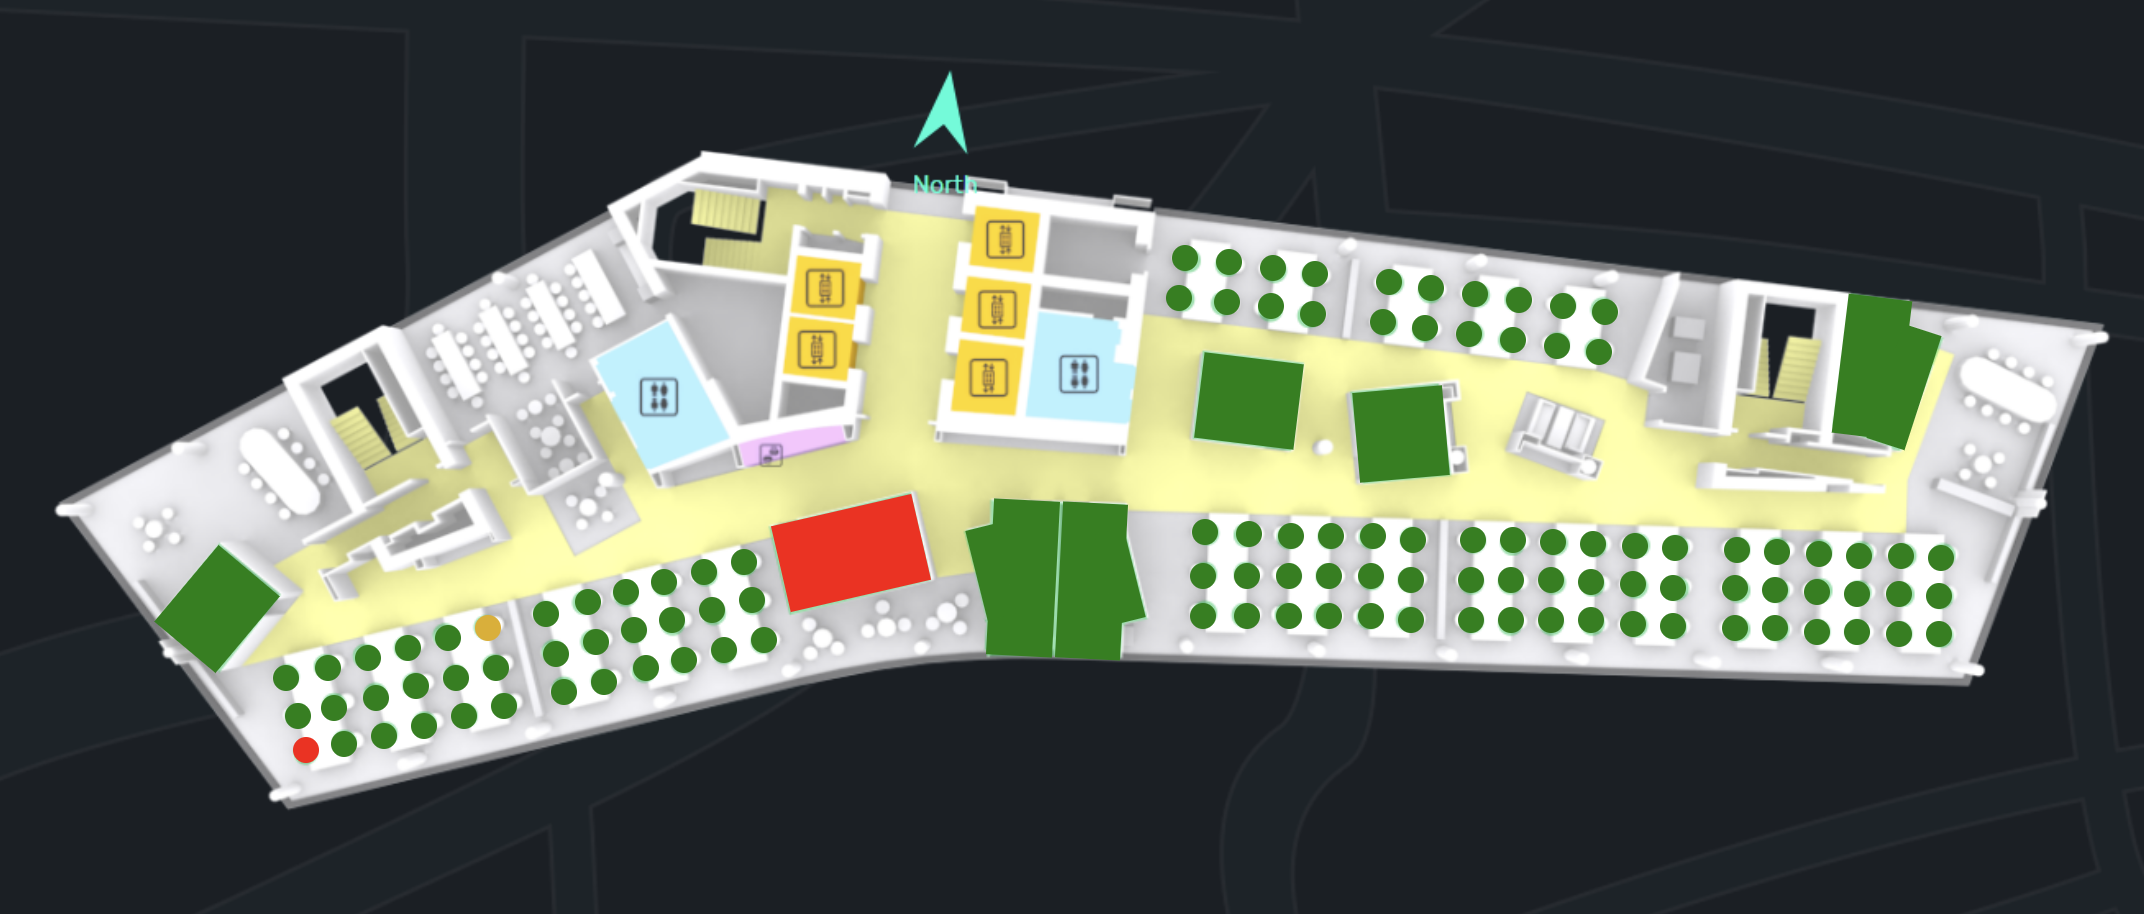
\includegraphics[width=0.9\linewidth]{images/sicily rezerv1.png}
    \caption{Sicily-6S rezervată între 09:30-10:30}
    \label{fig:sicily rezerv1.png}
\end{figure}

\begin{figure}[!htb]
    \centering
    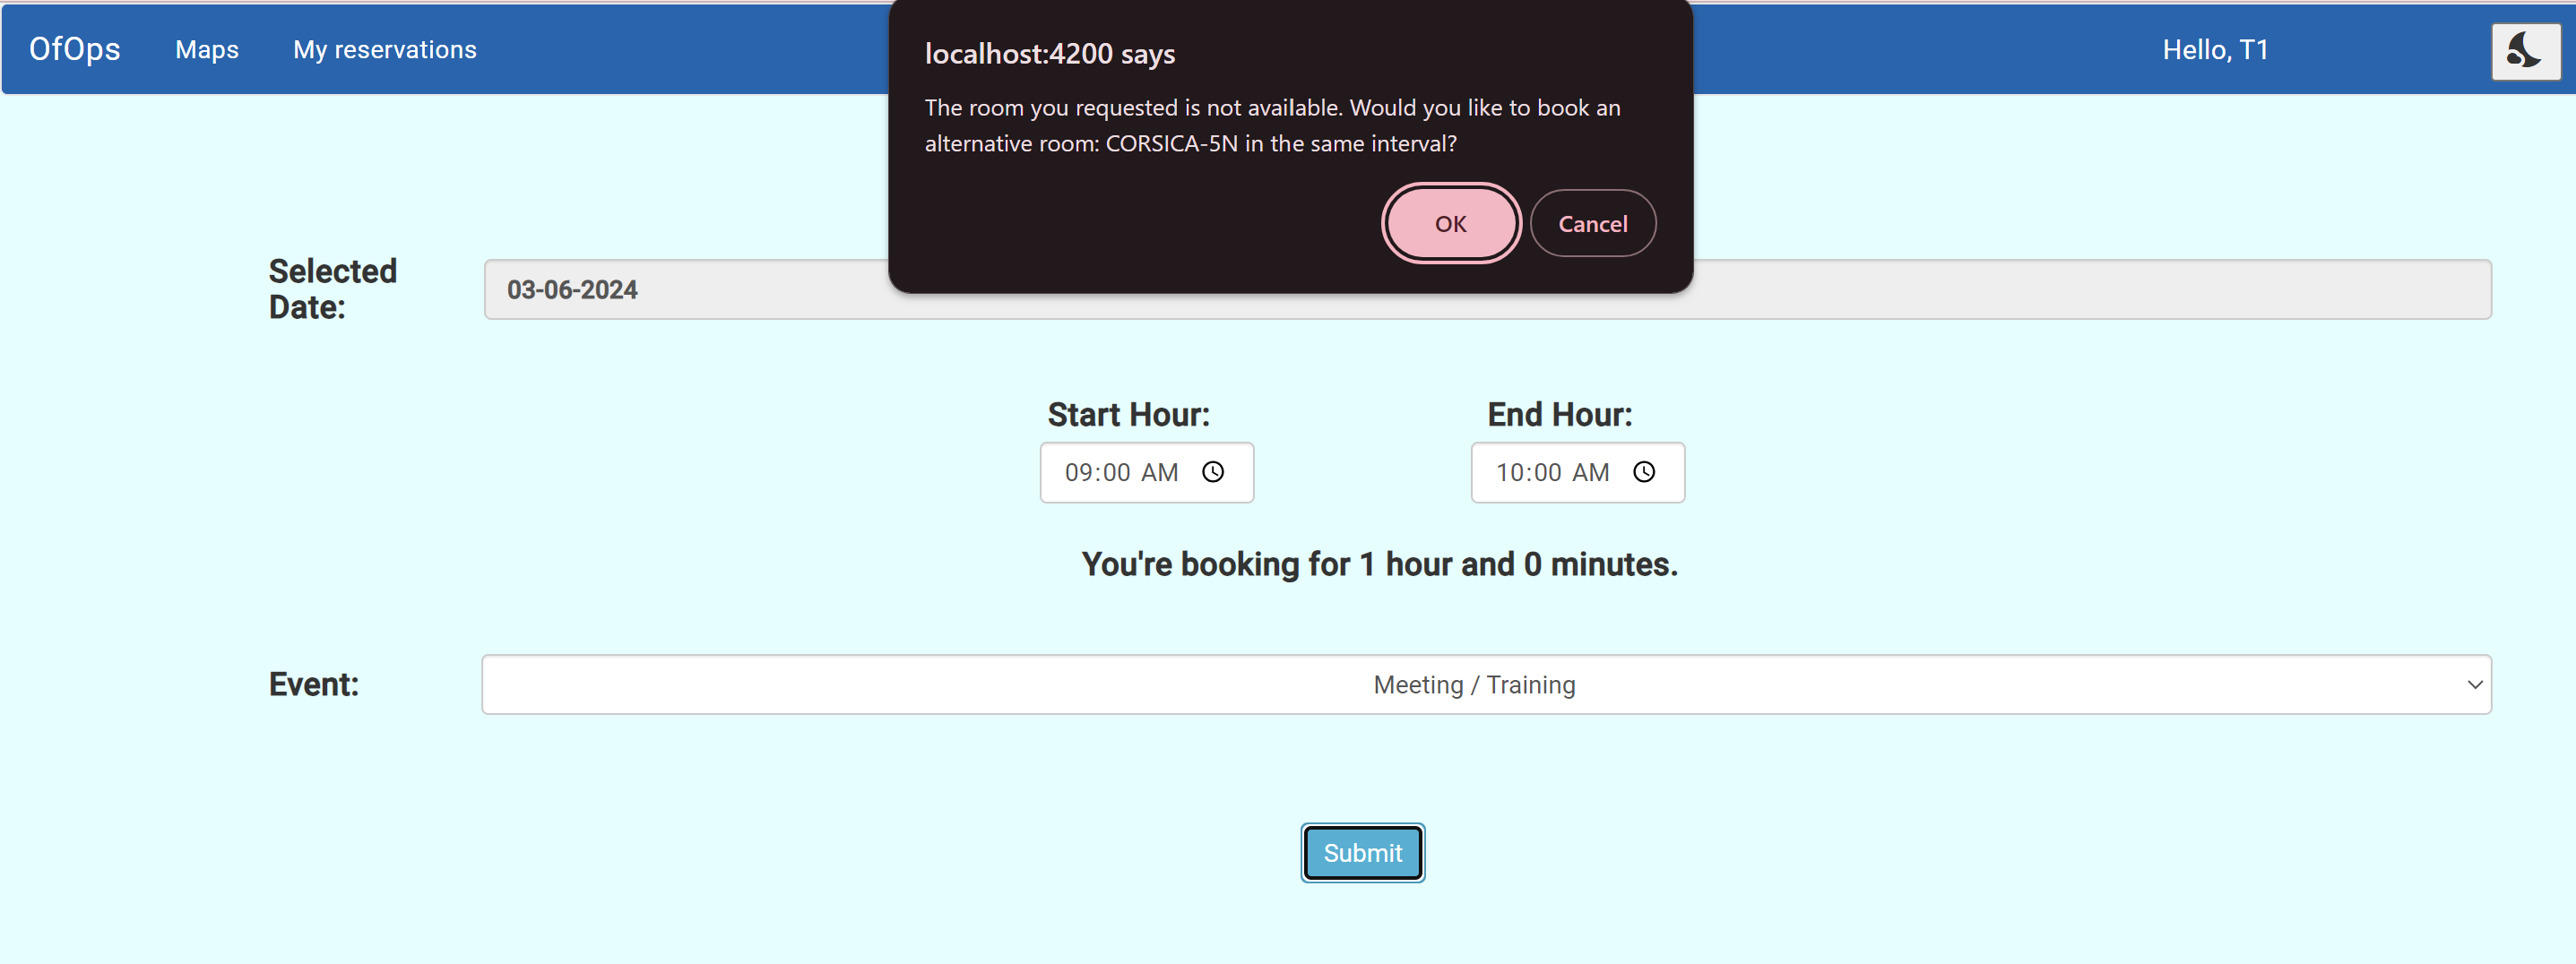
\includegraphics[width=0.9\linewidth]{images/sicily rezerv2.png}
    \caption{Propunerea de sală liberă în intervalul dorit}
    \label{fig:sicily rezerv2.png}
\end{figure}

Dacă răspunsul este afirmativ, utilizatorul primește o alertă cum că rezervarea sa a fost realizată cu succes.

\begin{figure}[!htb]
    \centering
    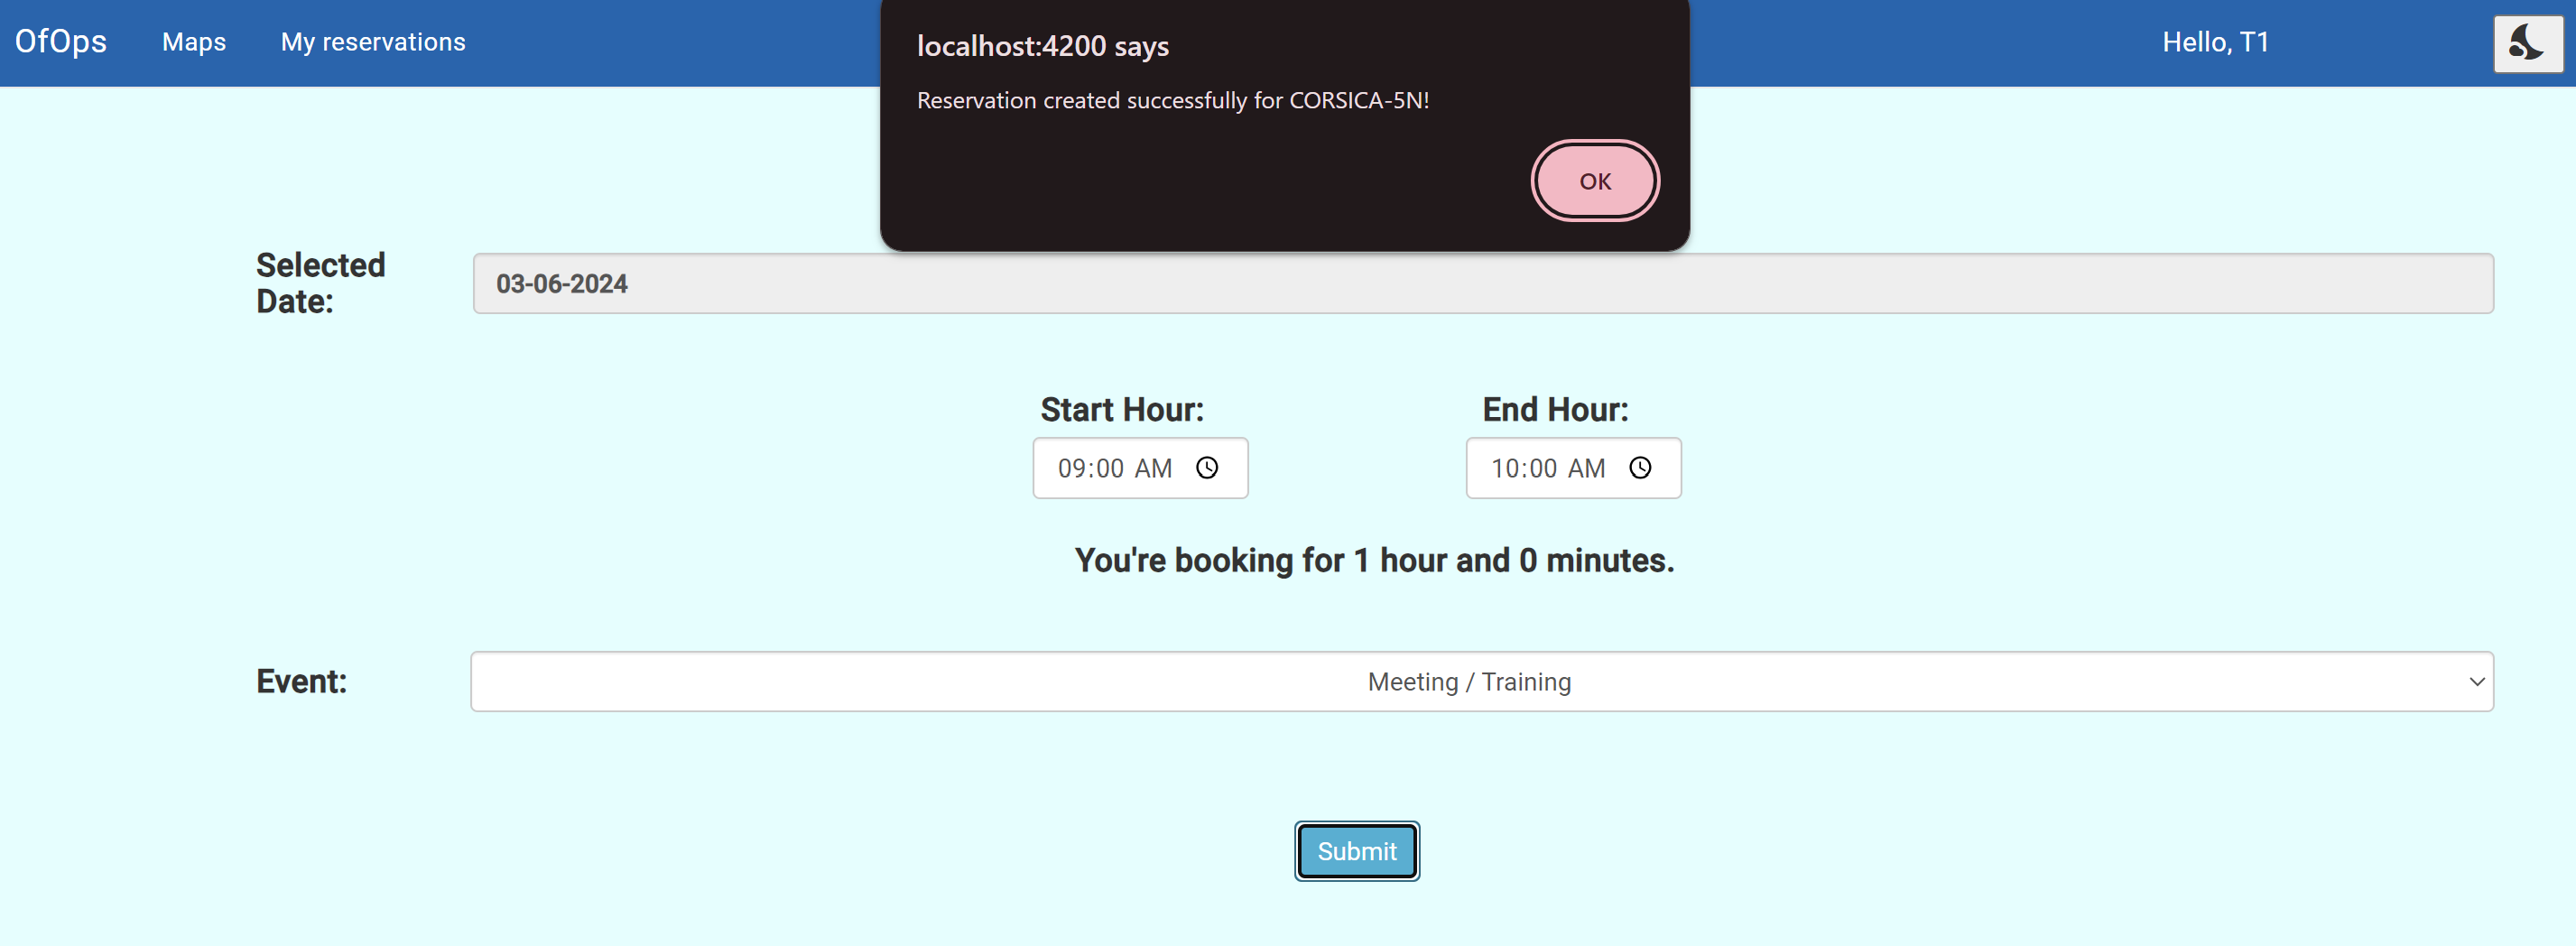
\includegraphics[width=0.9\linewidth]{images/sicily rezerv3.png}
    \caption{Rezervarea cu succes sălii propuse}
    \label{fig:sicily rezerv3.png}
\end{figure}

Astfel, user-ul va fi redirecționat către pagina de 
\textbf{My Reservations}.

\section{Pagina My Reservations}

Este pagina în care utilizatorul își poate vedea rezervările.

\begin{figure}[!htb]
    \centering
    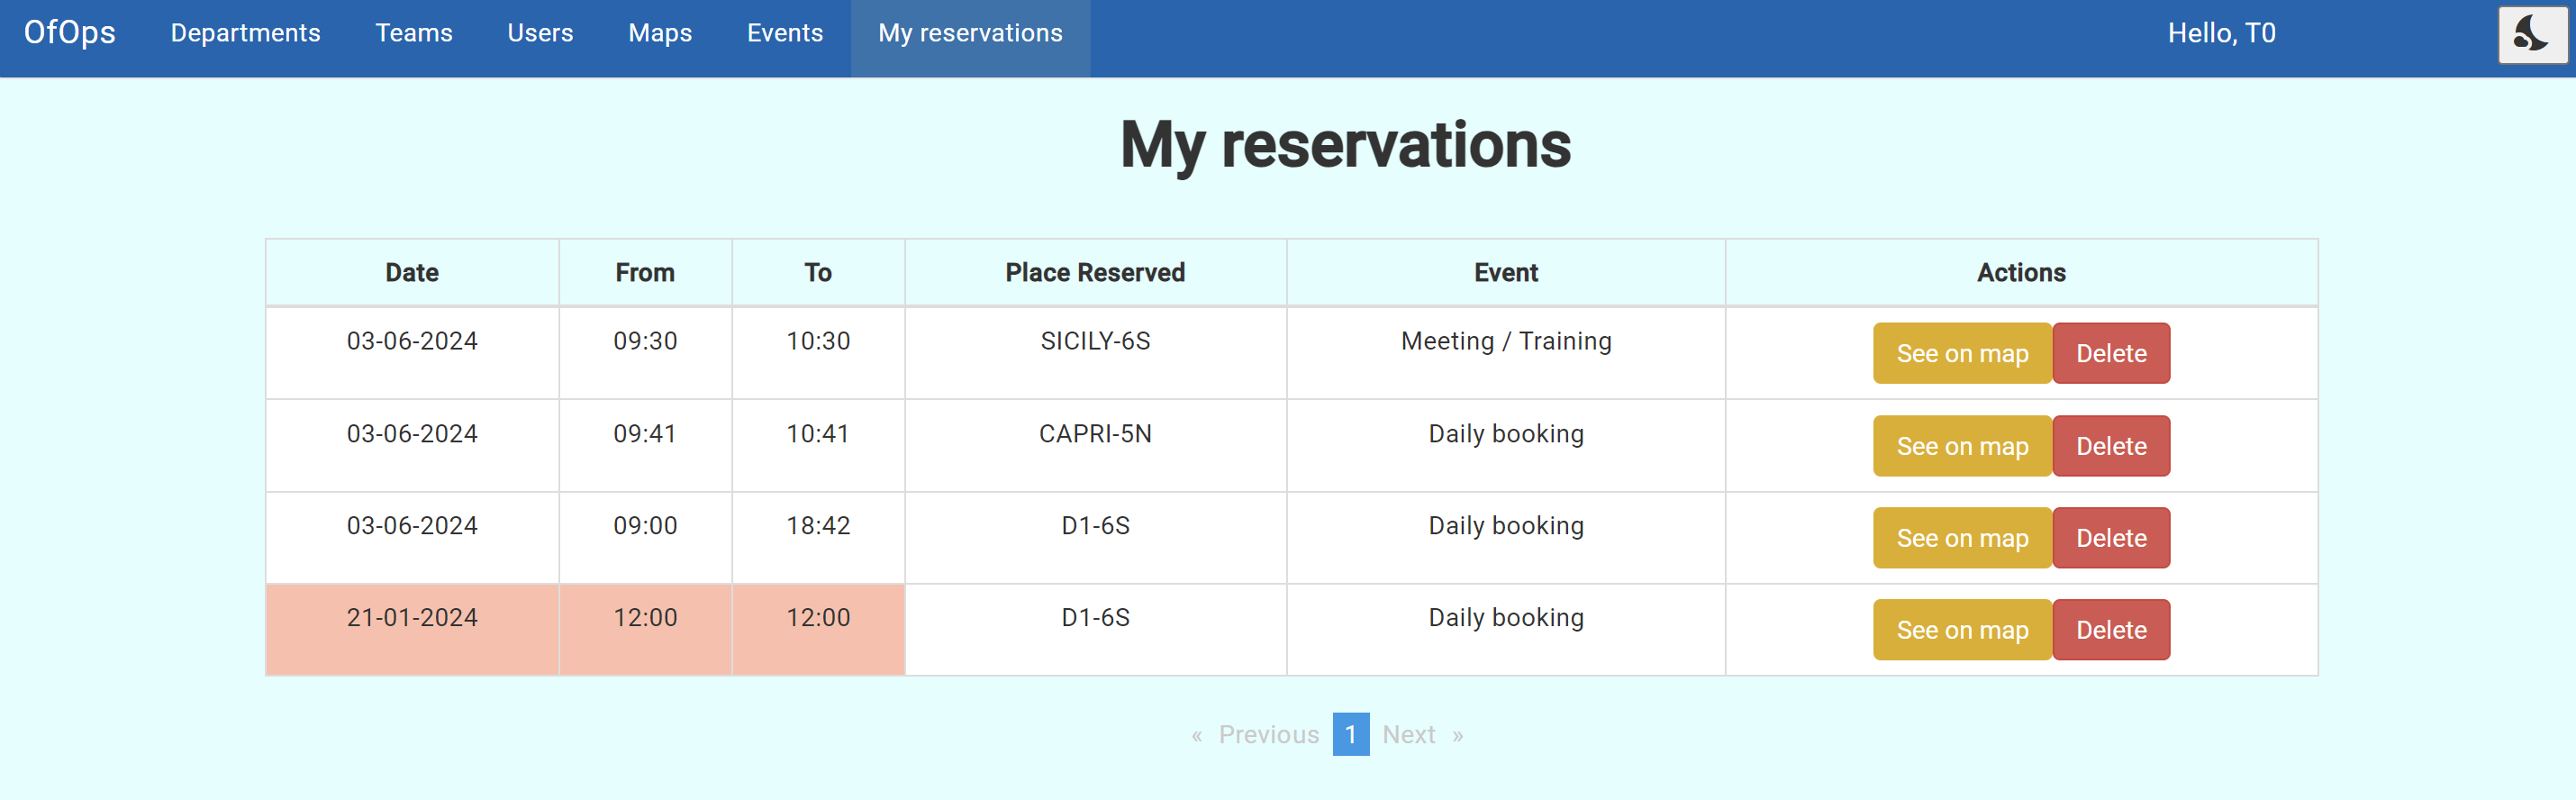
\includegraphics[width=0.9\linewidth]{images/myres.png}
    \caption{Pagina My reservations}
    \label{fig:myres}
\end{figure}

Aceasta are, de asemenea, introdusă și funcționalitatea de paginare, astfel încât gestionarea rezervărilor să fie o experiență plăcută pentru user, fără a-l încărca de informație.

Culoarea roșie a ultimei rezervări marchează faptul că aceasta este expirată, iar celelalte reprezintă viitoarele rezervări. Se poate observa că sunt prezente detaliile rezervărilor (data, orele de început și sfârșit, eventimentul pentru care sunt rezervate) și două butoane: \textbf{See on Map} și \textbf{Delete}.

\textbf{Delete} va șterge rezervarea, după dorința utilizatorului.

\begin{figure}[!htb]
    \centering
    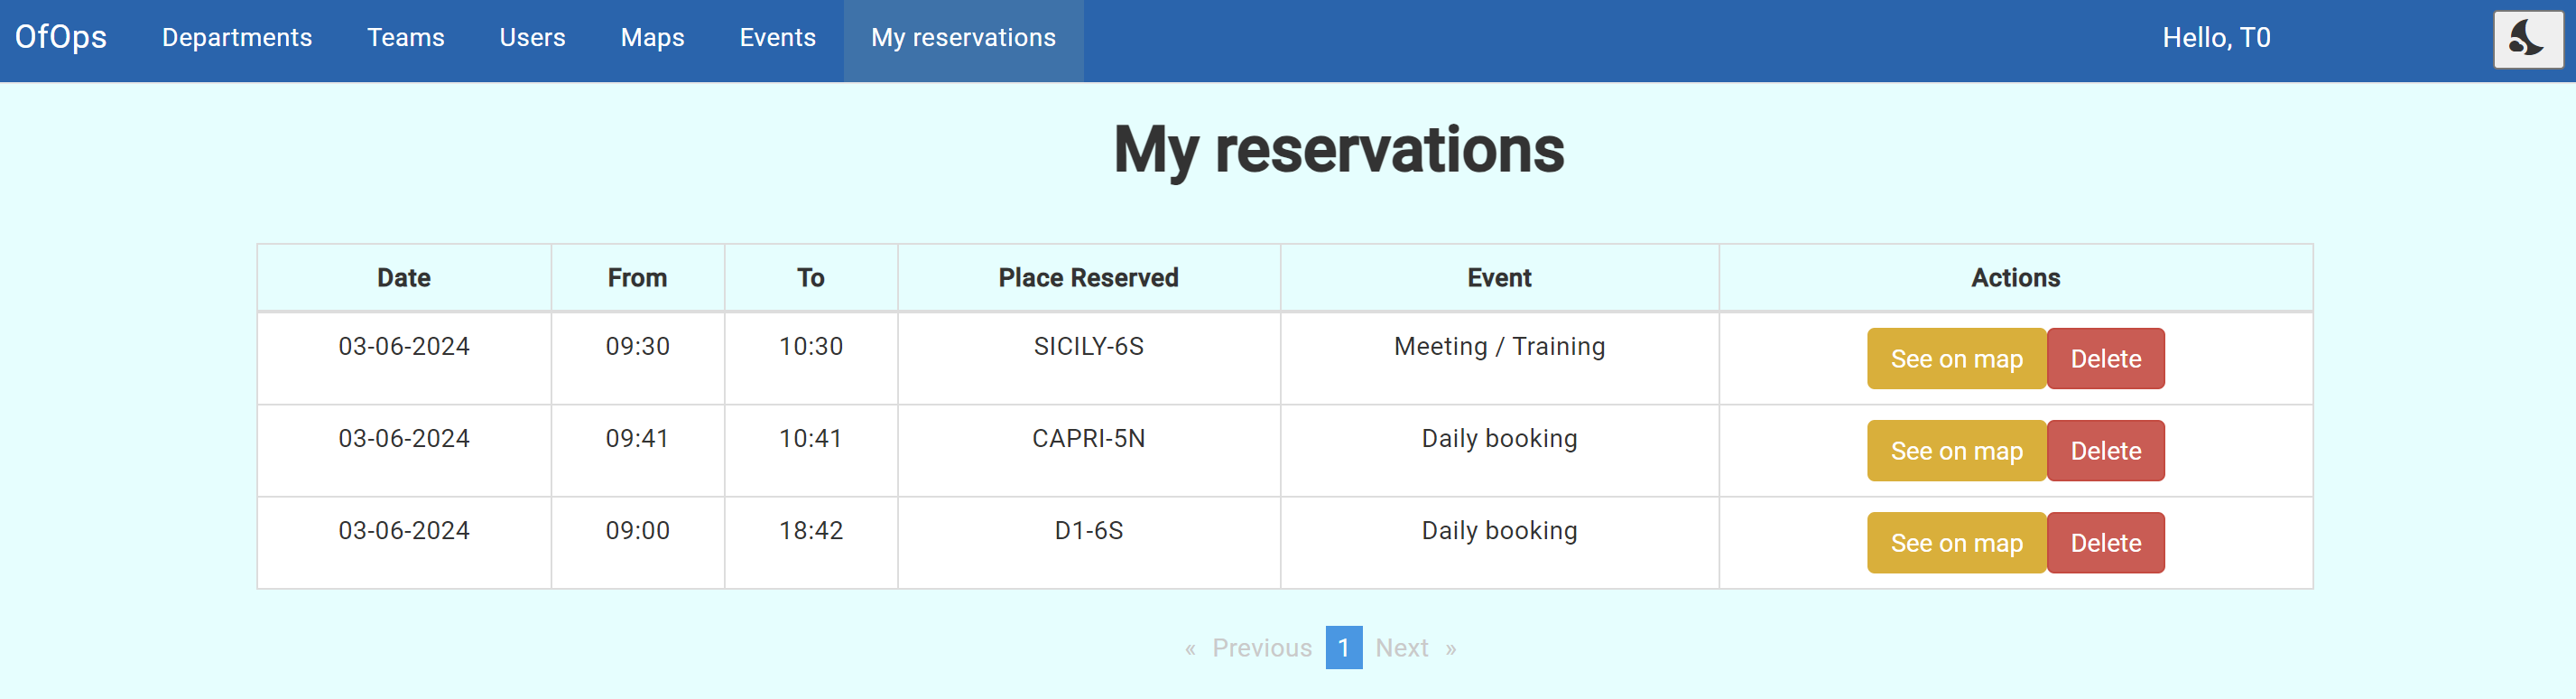
\includegraphics[width=0.9\linewidth]{images/delete.png}
    \caption{Ultima rezervare ștearsă}
    \label{fig:delete}
\end{figure}

Butonul \textbf{See on map} vine în ajutorul user-ului pentru a-și aduce aminte de locul rezervat. Acesta va fi redirecționat către harta și locul rezervat care va fi distins prin culoarea galbenă.

\begin{figure}[!htb]
    \centering
    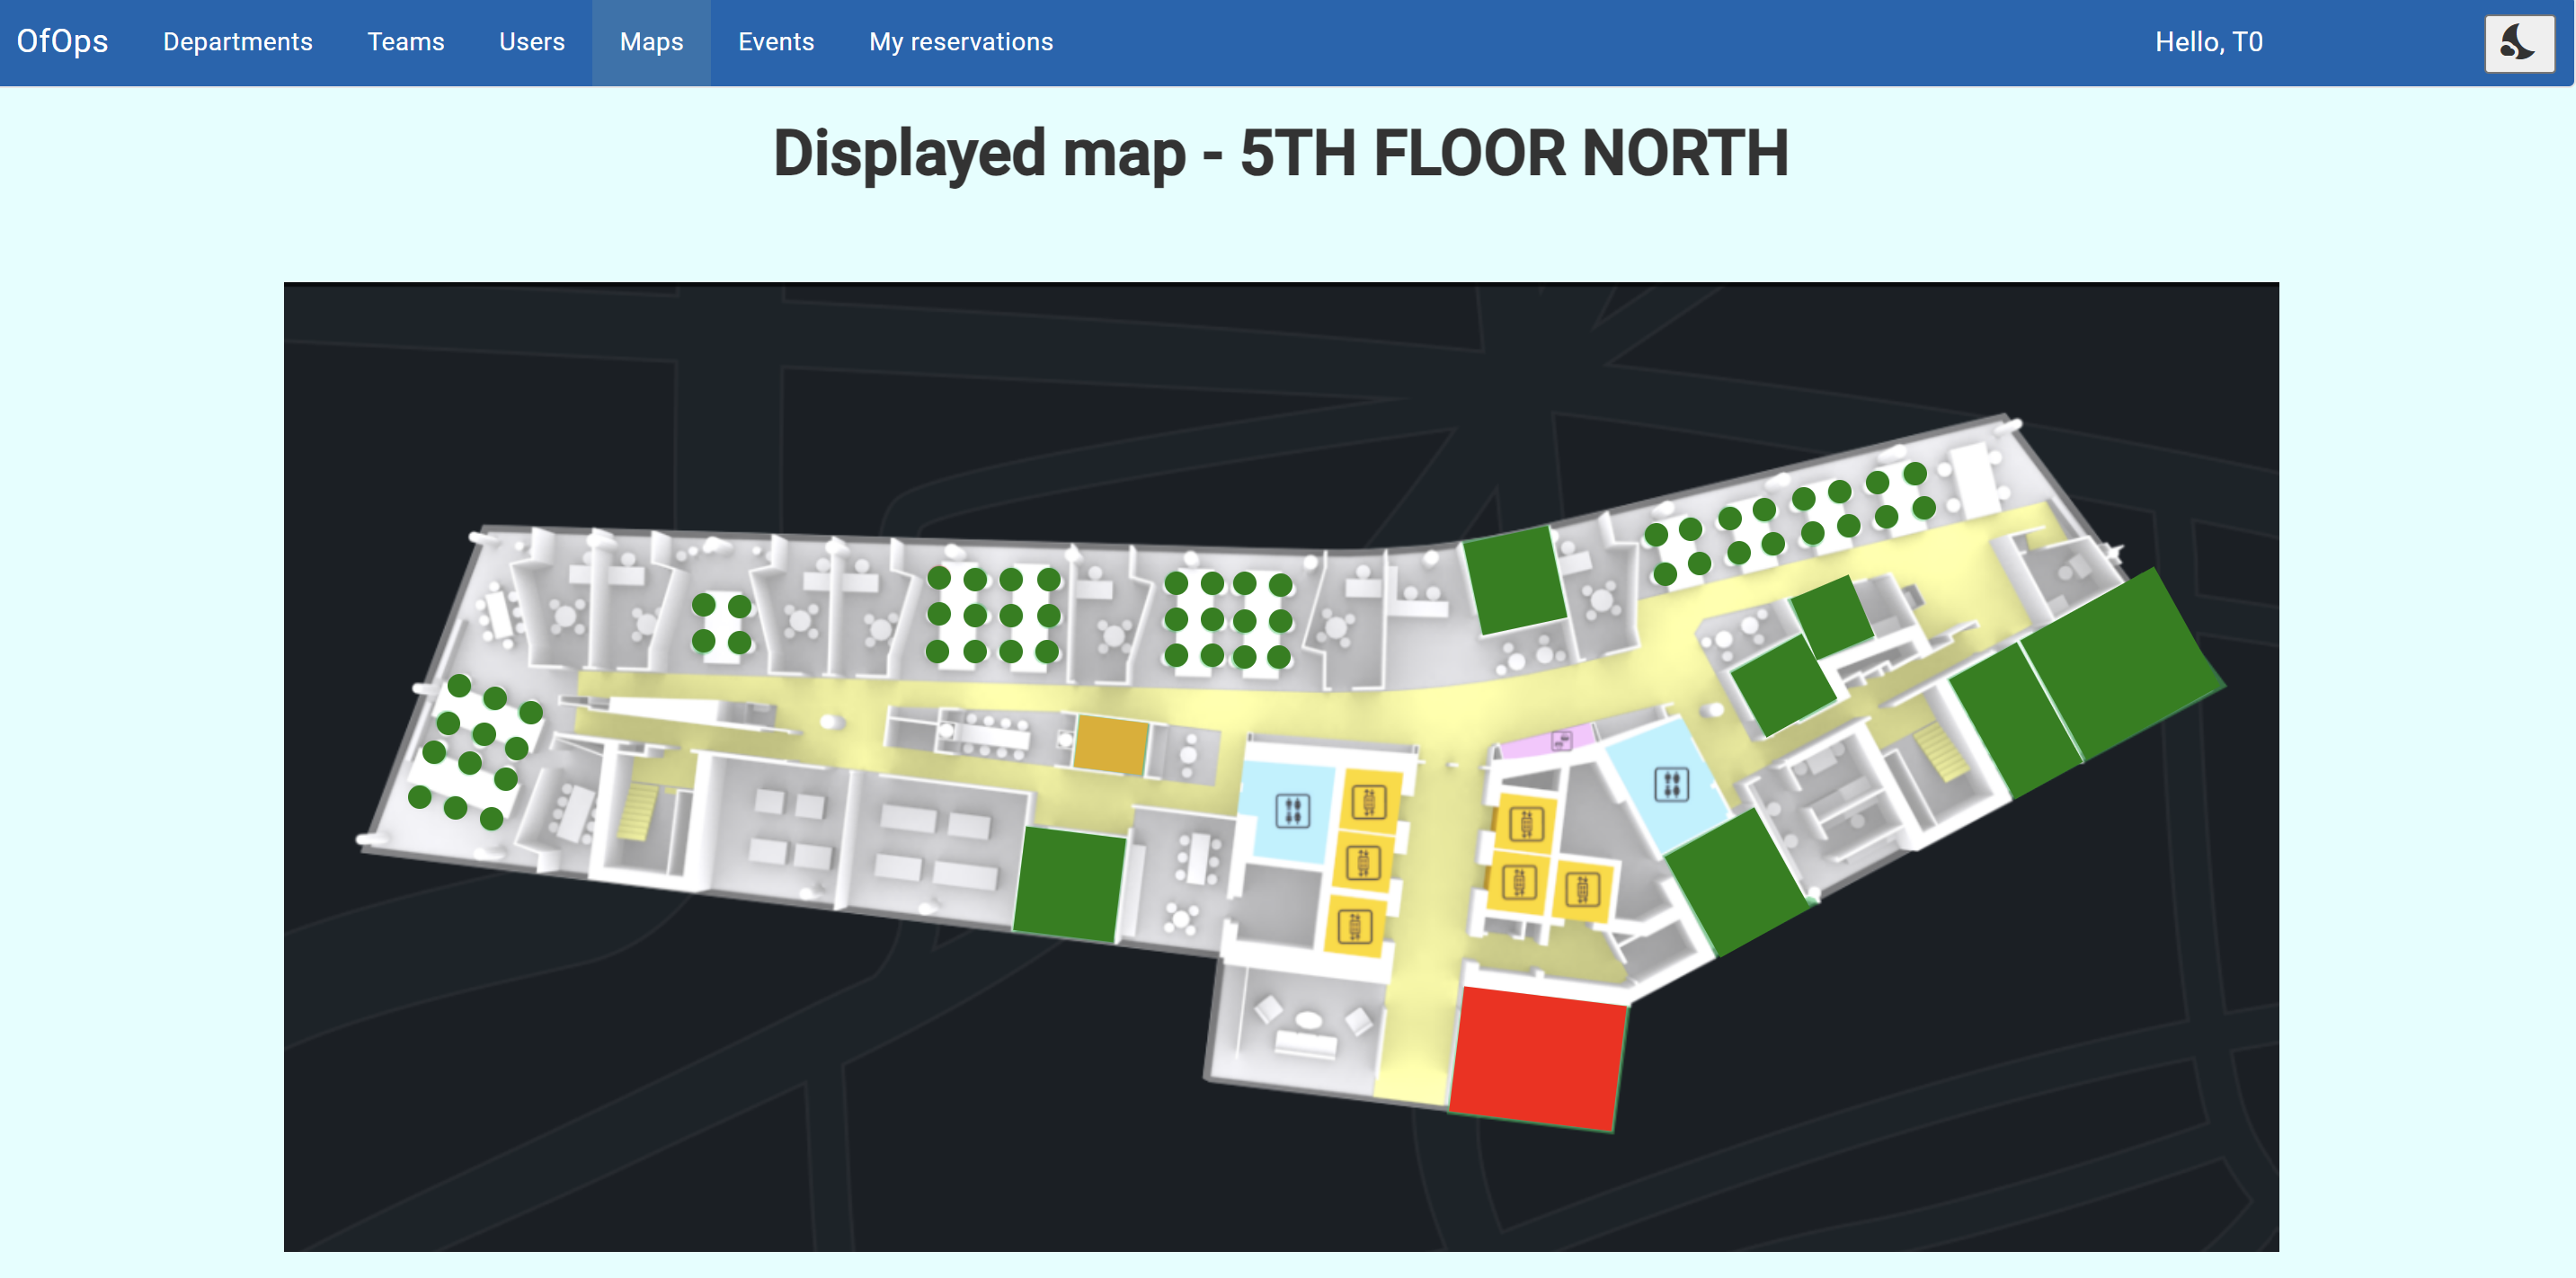
\includegraphics[width=0.9\linewidth]{images/rezerv utiliz.png}
    \caption{Rezervarea utilizatorului curent}
    \label{fig:rezerv utiliz}
\end{figure}

\section{Partea de ADMIN}